% Science of Remote Sensing (Elsevier) manuscript, elsarticle template. Written by paper_srs/build_main.py (numbers from the repository's CSV/LaTeX outputs).
% Compile: pdflatex main && bibtex main && pdflatex main && pdflatex main
\documentclass[preprint,12pt]{elsarticle}
\usepackage{amsmath}
\usepackage{booktabs}
\usepackage{array}
\usepackage{xcolor}
\usepackage{graphicx}
\usepackage{adjustbox}
\usepackage{algorithm}
\usepackage{algpseudocode}
\usepackage{placeins}
\usepackage{lineno}
\usepackage[colorlinks=true,allcolors=blue!50!black]{hyperref}
\modulolinenumbers[5]
\newcommand{\dinoseg}{StrongDINOv2Seg}
\newcommand{\Lcost}{L_{\mathrm{cost}}}
\newcommand{\pending}[1]{\textcolor{red}{\textit{#1}}}
\algrenewcommand\algorithmicrequire{\textbf{Input:}}
\algrenewcommand\algorithmicensure{\textbf{Output:}}
\algrenewcommand\alglinenumber[1]{\scriptsize #1:}
\setlength{\emergencystretch}{2em}
\hfuzz=3pt\vfuzz=10pt   % elsarticle's own preprint title-page footer is 2.6 pt wide / 7.5 pt high in a minimal document too; nothing else exceeds the page
\renewcommand{\topfraction}{0.9}\renewcommand{\textfraction}{0.08}\renewcommand{\floatpagefraction}{0.7}
\biboptions{sort&compress}
\journal{Science of Remote Sensing}
\begin{document}
\linenumbers
\begin{frontmatter}
\title{Propagating open building-footprint uncertainty into shared rural road networks: a four-window study in Telangana, India}
\author[cbit]{Pendyala Archana}
\author[cbit]{Ramakrishna Kolikipogu\corref{cor1}}
\cortext[cor1]{Corresponding author.}
\affiliation[cbit]{organization={Department of Information Technology, Chaitanya Bharathi Institute of Technology (A)},city={Hyderabad},country={India}}
\begin{highlights}
\item Open-data pipeline turns building footprints into shared rural road plans
\item Shared networks are 12.2-25.3\% shorter than independent routes in four windows
\item Footprint detection precision 0.89-0.95, but 40-52\% merge several buildings
\item Omitting 20\% of footprints leaves households unserved, not networks oversized
\item Kou Steiner baseline is only 0.6-3.2\% longer than the shared plan
\end{highlights}
\begin{graphicalabstract}
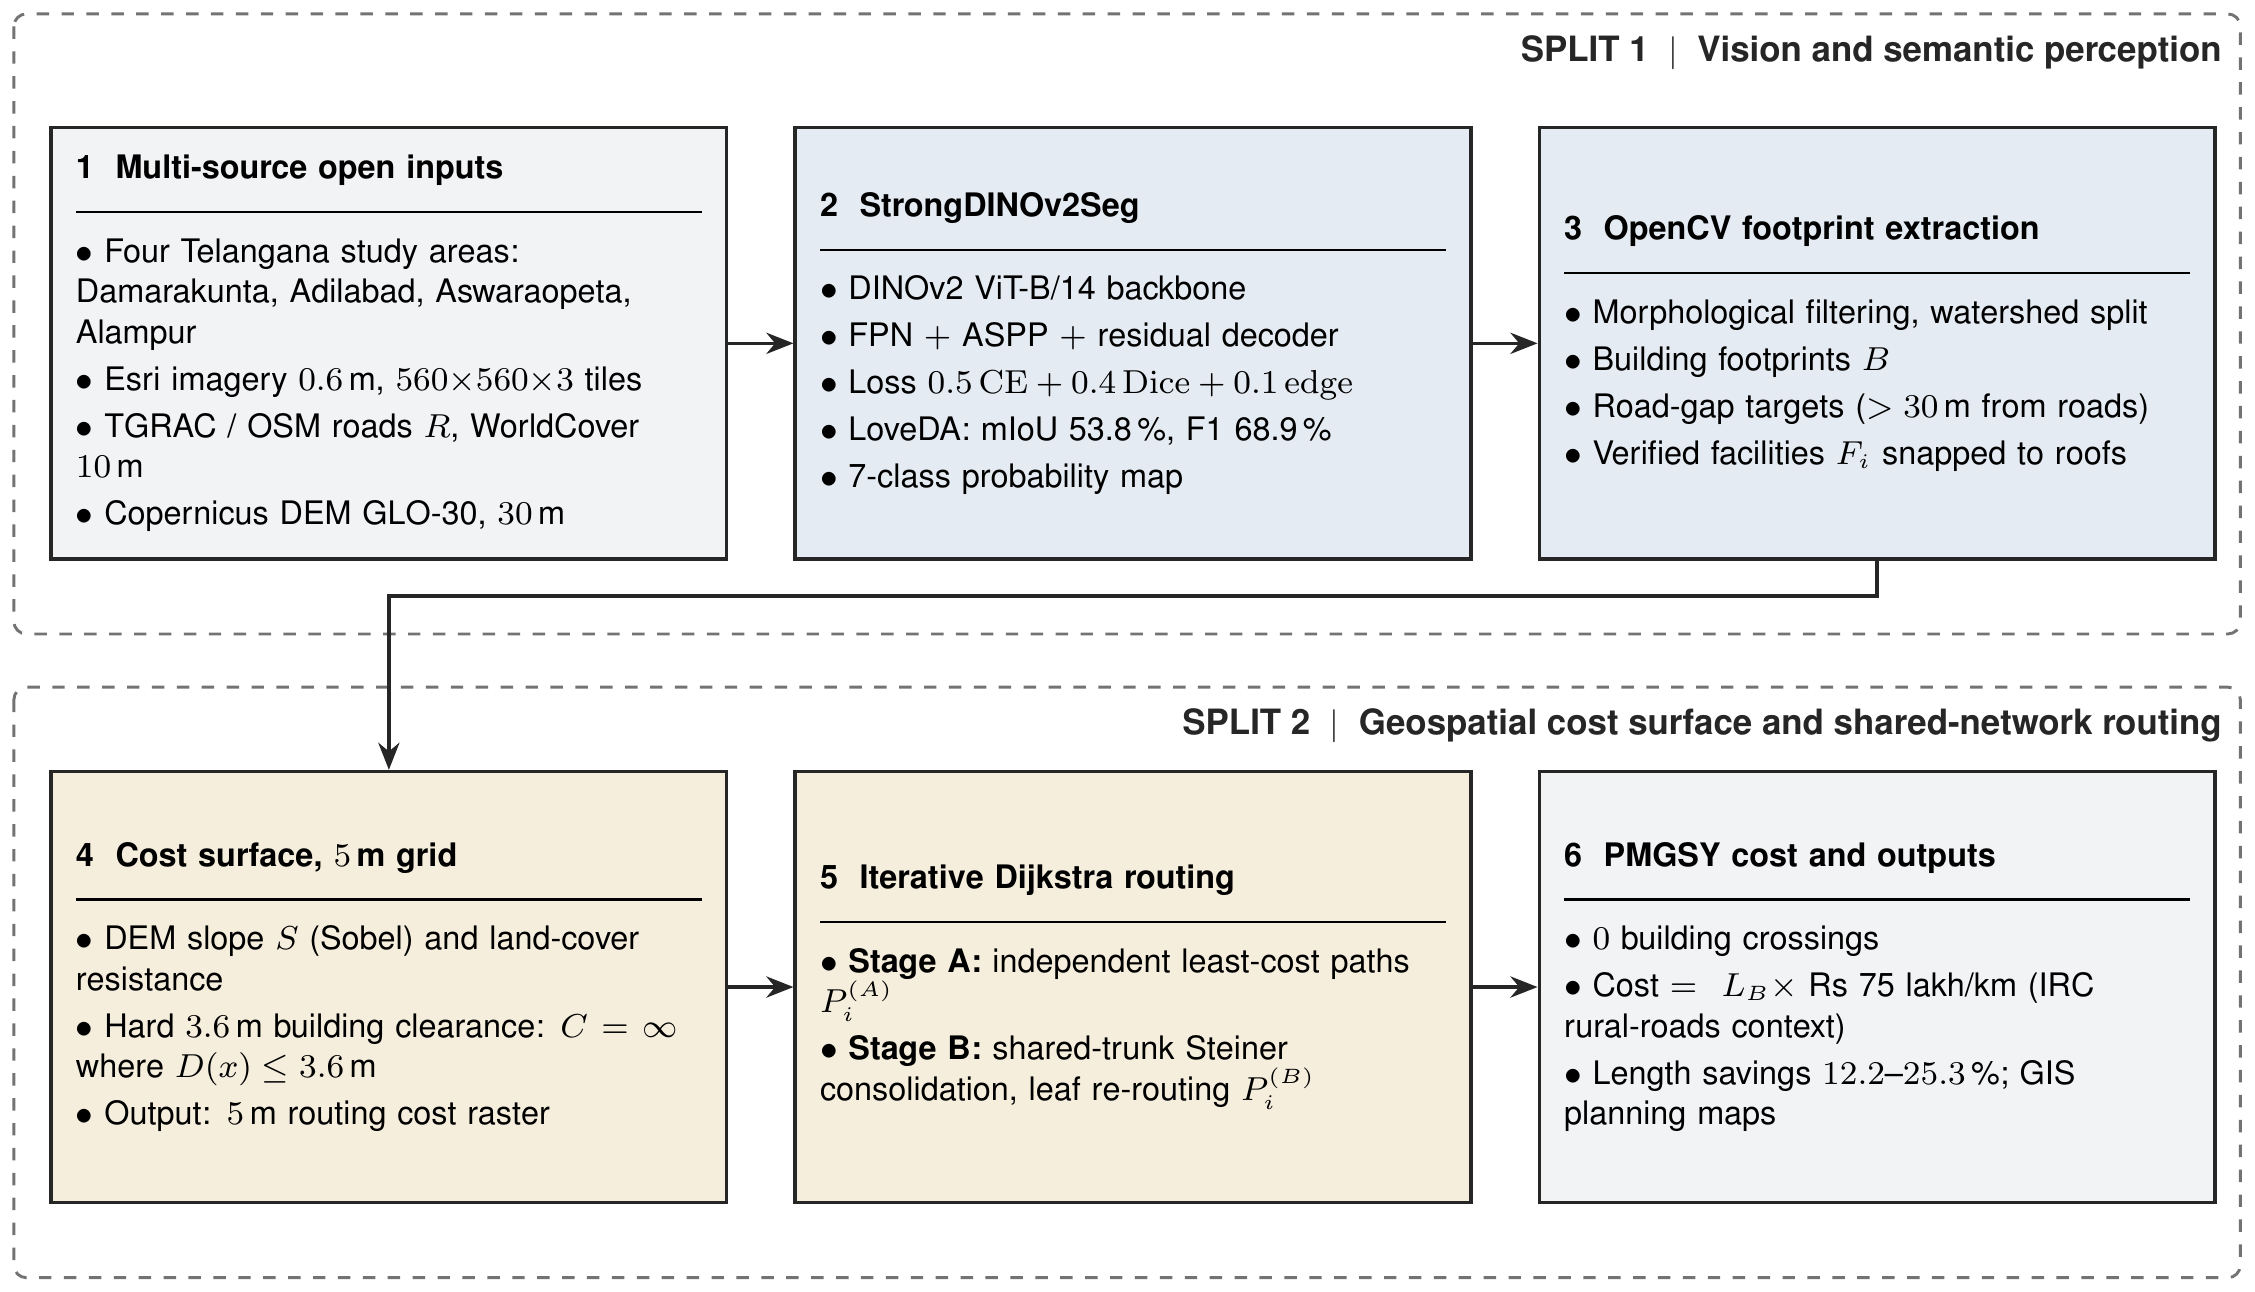
\includegraphics[width=\textwidth]{graphical_abstract.png}
\end{graphicalabstract}
\begin{abstract}
Planning access roads for unconnected rural buildings with open Earth-observation data inherits the errors of the building inventory, yet these errors are seldom propagated to the plan. We apply one fully open workflow to four Telangana windows (0.46--18.59~km$^2$): a frozen segmenter, StrongDINOv2Seg (53.8\% mean intersection over union, mIoU, on the LoveDA benchmark), applied to 0.6~m Esri imagery gives building footprints and road-gap targets; land cover and terrain slope give a multi-criteria cost surface on a 5~m grid with a hard 3.6~m building clearance; and two-stage Dijkstra routing consolidates independent routes into a shared network. The shared network is 12.2 to 25.3\% shorter than independent routes, with zero building crossings in all four windows. We then test the weakest input without manual labels. Against Overture Maps buildings the footprints reach an area overlap (intersection over union, IoU) of 0.283 to 0.373 and a detection precision of 0.893 to 0.950, but 40 to 52\% of them merge two or more reference buildings. Omitting 20\% of the road-gap footprints leaves 5 to 169 households unserved while the length per served household changes little, and a Kou Steiner tree is 0.6 to 3.2\% longer than the shared plan. The results are agreement and sensitivity figures between open datasets, not accuracy against field ground truth, and the corridors are planning alternatives for field verification.
\end{abstract}
\begin{keyword}
rural roads\sep building footprint extraction\sep satellite remote sensing\sep uncertainty propagation\sep least-cost path\sep Steiner tree\sep open geospatial data
\end{keyword}
\end{frontmatter}

\section{Introduction}
\section{Introduction}
Road building is among the most consequential land-use changes of the coming decades. Global road length is projected to grow by roughly 3.0--4.7 million km by 2050 \cite{meijer2018global}, and new roads open land to clearing, fragmentation and conversion \cite{laurance2014global}. Much of this growth is local. In India the Pradhan Mantri Gram Sadak Yojana (PMGSY) connects habitations through all-weather rural roads \cite{pmgsy}, and planning for such schemes depends on knowing where dwellings and facilities are, what terrain and land cover a corridor must cross, and which connection rule is applied.

Computational support for this planning has matured along three separate lines. Remote sensing now maps buildings and roads at large scale, from continental building inventories \cite{sirko2021openbuildings} to foundation-model segmenters \cite{oquab2023dinov2}, with recent work on small and isolated rural buildings, uncertainty and domain shift \cite{r62,r63,r64,r65,r66,r67,r68,r69,r70}, on road extraction for rural and arid scenes \cite{r56,r57,r58,r59,r60} and on informal settlements \cite{r48}. Multi-criteria and least-cost analysis translates terrain and land cover into route costs \cite{r06,r53,r54,collischonn2000lcp}. Network-design formulations connect many demand points at low total cost, including Steiner-tree heuristics \cite{kou1981steiner,mehlhorn1988steiner,hwang1992steiner,r51}, rural road design models \cite{r41,r43,r44} and analogues for power and transport networks \cite{r45,r46,r47,r50}. These lines are rarely joined: detectors are judged by pixel overlap \cite{r01,foody2002status}, planners assume an error-free inventory \cite{heuvelink1998error}, and each house is often connected independently, so neighbouring houses re-trace the same corridor. To our knowledge no cited work combines satellite-derived building instances, a land-cover and slope cost surface with building avoidance, and a shared-network planner whose marginal cost credits built corridors.

We therefore ask not only whether shared rural road networks can be planned from open Earth-observation data, but how far such a plan can be trusted when the building inventory it rests on is incomplete or merged. We join the three lines in one two-split framework (figure~\ref{fig:arch}) and apply it, unchanged, to four settlement windows of different morphology in Telangana, built from one set of open data layers and one frozen segmentation checkpoint. Our objectives are (1)~to develop a reproducible framework whose first split extracts building footprints, road-gap targets and verified facilities from open imagery and whose second split builds a terrain and land-cover cost surface with a hard building clearance and consolidates independent routes into a shared network; (2)~to test whether the same checkpoint and rules transfer without retraining across a rural village, an urban fringe, a semi-urban town and a heritage town; (3)~to quantify the length, cost and building-crossing outcomes of independent (Stage~A) and shared (Stage~B) routing against baseline strategies; and (4)~to report, with automated multi-source checks and no manual labelling, how closely the footprints agree with open building inventories, how footprint omission propagates into network length and unserved households, and how the shared plan compares with a Kou Steiner tree and a Euclidean minimum spanning tree.

\section{Data and methods}\label{sec:data}
\subsection{Selection and characteristics of the four Telangana study windows}
The four windows span the settlement gradient of Telangana from a dispersed village to a district town (figure~\ref{fig:flow}), so that the same method meets different building densities, road coverage and facility mixes. All use UTM zone 44N (EPSG:32644) and the same open data stack (table~\ref{tab:data}). Because no official village or town polygon was available for them, each study window is the built-up settlement extent derived from open data around the settlement centre, with an edge-continuity check against ESA WorldCover; the windows are therefore settlement extents, not administrative polygons.

\textbf{Damarakunta} (Siddipet district, Markook mandal; $17.707^{\circ}$N, $78.753^{\circ}$E) is a dispersed rural village whose houses cluster around one core. Its window is the extent derived from Overture building footprints around the village centre (the footprints themselves come from the segmentation). The window covers 0.46~km$^2$ with 3.5~km of mapped road and a mean slope of 3.8\%. The segmenter yields 100 building instances (\textsc{Plausible} 44, \textsc{Review} 11, \textsc{Unresolved\_Merge} 40, and 5 smaller than 30~m$^2$), of which 27 lie more than 30~m from a road and become targets. The audit retains 2 verified facilities (1 hospital or health centre and 1 anganwadi). 

\textbf{Adilabad} (Adilabad district; $19.676^{\circ}$N, $78.534^{\circ}$E) is the urban fringe of the district town. Its window is the built-up extent derived from ESA WorldCover around the OpenStreetMap place node, spanning the Adilabad Urban mandal (50.5\%), Mavala (32.2\%) and Adilabad Rural (17.4\%). It is the largest window and has the densest fabric. It covers 18.59~km$^2$ with 509.9~km of mapped road and a mean slope of 3.1\%. The segmenter yields 5{,}653 building instances (\textsc{Plausible} 2{,}526, \textsc{Review} 181, \textsc{Unresolved\_Merge} 2{,}773, and 173 smaller than 30~m$^2$), of which 613 lie more than 30~m from a road and become targets. The audit retains 132 verified facilities (39 schools, 15 colleges, 59 hospitals and health centres, 15 government offices and 4 anganwadis). 

\textbf{Aswaraopeta} (Bhadradri Kothagudem district; $17.241^{\circ}$N, $81.128^{\circ}$E) is the headquarters town of Aswaraopeta mandal, a semi-urban tribal-fringe town. Its window is the WorldCover built-up extent around the Overture locality point.  It covers 2.82~km$^2$ with 28.6~km of mapped road and a mean slope of 3.1\%. The segmenter yields 1{,}297 building instances (\textsc{Plausible} 772, \textsc{Review} 18, \textsc{Unresolved\_Merge} 452, and 55 smaller than 30~m$^2$), of which 678 lie more than 30~m from a road and become targets. The audit retains 32 verified facilities (5 schools, 3 colleges, 7 hospitals and health centres, 3 government offices and 14 anganwadis). 

\textbf{Alampur} (Jogulamba Gadwal district; $15.880^{\circ}$N, $78.135^{\circ}$E) is a small heritage town on the Tungabhadra, known for its temple complex. Its window is the extent derived from Overture building footprints around the OpenStreetMap place node.  It covers 1.65~km$^2$ with 25.3~km of mapped road and a mean slope of 2.1\%. The segmenter yields 430 building instances (\textsc{Plausible} 208, \textsc{Review} 26, \textsc{Unresolved\_Merge} 163, and 33 smaller than 30~m$^2$), of which 59 lie more than 30~m from a road and become targets. The audit retains 9 verified facilities (1 school, 1 college, 2 hospitals and health centres and 5 anganwadis). 

\subsection{Datasets}
All four windows are processed from the same open layers (table~\ref{tab:areas}): 0.6~m Esri World Imagery, \dinoseg{} building footprints, ESA WorldCover v200 land cover ($10$~m), the Copernicus GLO-30 elevation model ($30$~m), Overture Maps and OpenStreetMap road networks, and verified public facilities from OpenStreetMap, Overture Places, Wikidata \cite{vrandecic2014wikidata} and Wikipedia. The training benchmark is LoveDA, from which one checkpoint serves all windows. No layer is specific to one window. \emph{Data vintage.} Overture layers come from the pinned release 2026-10-21.0 (the release of 2026-11-18.0 is newer and not used). OpenStreetMap (Overpass, Photon), Wikidata and Wikipedia were queried live on 2026-11-25 (Adilabad, Aswaraopeta, Alampur) and 2026-11-26 (Damarakunta), and every answer is cached per query. The Esri service metadata gives Vantor Vivid imagery at 0.34~m captured on 2026-04-29 (Damarakunta), 2025-01-26 (Adilabad), 2025-12-10 (Aswaraopeta) and 2026-02-16 (Alampur); the footprints come from earlier mosaic exports (before 2026-11-03 for Damarakunta) whose imagery version was not recorded. WorldCover (version 200, 2021) and the Copernicus GLO-30 tiles are static.

\begin{table}[t]
\caption{The four study windows and the data layers of each; the layers are the same open sources in every window. Top: window profiles (road length is the mapped road layer inside the window; slope is the mean terrain slope). Middle: the layer used in each window (OSM: OpenStreetMap; WorldCover: ESA WorldCover land-cover map; DEM: digital elevation model; GLO-30: Copernicus global 30~m DEM; LoveDA: Land-cover Domain Adaptive semantic segmentation dataset; ODbL: Open Database Licence; CC BY: Creative Commons Attribution). Bottom: the datasets with resolution, version, licence and location.}
\label{tab:areas}\label{tab:data}
\centering
\scriptsize
\renewcommand{\arraystretch}{1.1}
\begin{adjustbox}{max width=\textwidth}
\begin{tabular}{@{}>{\raggedright\arraybackslash}p{2.3cm}>{\raggedright\arraybackslash}p{3.2cm}>{\raggedright\arraybackslash}p{3.2cm}>{\raggedright\arraybackslash}p{3.2cm}>{\raggedright\arraybackslash}p{3.2cm}@{}}
\toprule
 & Damarakunta & Adilabad & Aswaraopeta & Alampur\\
\midrule
District & Siddipet & Adilabad & Bhadradri Kothagudem & Jogulamba Gadwal\\
Typology & Rural & Urban fringe & Semi-urban, tribal fringe & Heritage, semi-urban\\
Window (km$^2$) & 0.46 & 18.59 & 2.82 & 1.65\\
Existing roads (km) & 3.5 & 509.9 & 28.6 & 25.3\\
Mean slope (\%) & 3.8 & 3.1 & 3.1 & 2.1\\
\midrule
Boundary & Built-up extent from Overture footprints around the village centre & Built-up extent from WorldCover around the OSM place node & Built-up extent from WorldCover around the Overture locality point & Built-up extent from Overture footprints around the OSM place node\\
Existing roads & \multicolumn{4}{@{}l}{Overture Maps and OSM road networks (all four windows)}\\
Public facilities & 2 verified & 132 verified & 32 verified & 9 verified\\
Building footprints & \multicolumn{4}{@{}l}{\dinoseg{} on 0.6~m Esri imagery: 100, 5{,}653, 1{,}297, 430 instances}\\
Land cover & \multicolumn{4}{@{}l}{ESA WorldCover, 10~m, v200}\\
Terrain & \multicolumn{4}{@{}l}{Copernicus DEM GLO-30, 30~m, slope by the Sobel method}\\
Training benchmark & \multicolumn{4}{@{}l}{LoveDA, one checkpoint for all four windows}\\
\bottomrule
\end{tabular}
\end{adjustbox}

\medskip
\begin{adjustbox}{max width=\textwidth}
\begin{tabular}{@{}>{\raggedright\arraybackslash}p{3.4cm}>{\raggedright\arraybackslash}p{1.7cm}>{\raggedright\arraybackslash}p{1.8cm}>{\raggedright\arraybackslash}p{3.0cm}>{\raggedright\arraybackslash}p{5.0cm}@{}}
\toprule
Dataset (use) & Resolution & Version & Licence & URL / DOI\\
\midrule
Esri World Imagery \cite{esri2026worldimagery} (imagery) & 0.6~m & live service; captures 2025-01 to 2026-04 & Esri terms; academic use, credit required & \url{services.arcgisonline.com/ArcGIS/rest/services/World_Imagery/MapServer}\\
Overture Maps \cite{overture2026} (roads, places, footprints for window extents) & vector & 2026-10-21.0 (pinned) & ODbL 1.0; CDLA-Permissive-2.0 & \url{overturemaps.org}\\
OpenStreetMap \cite{haklay2008osm} (roads, facilities) & vector & live; queried 2026-11-25/26 & ODbL 1.0 & \url{openstreetmap.org/copyright}\\
ESA WorldCover \cite{zanaga2021worldcover} (land cover) & 10~m & v200 (2021), static & CC BY 4.0 & \url{doi.org/10.5281/zenodo.7254221}\\
Copernicus DEM GLO-30 \cite{esa2022copdem} (slope) & 30~m, slope at 10~m & GLO-30 COG, file dated 2022-05-09 & Copernicus licence & \url{doi.org/10.5270/ESA-c5d3d65}\\
LoveDA \cite{wang2021loveda} (training, validation) & 0.3~m & 2021 & CC BY-NC-SA 4.0 & \url{doi.org/10.5281/zenodo.5706578}\\
Wikidata \cite{vrandecic2014wikidata}, Wikipedia (facility audit) & points & live; queried 2026-11-25/26 & CC0; CC BY-SA 4.0 & \url{wikidata.org}\\
\bottomrule
\end{tabular}
\end{adjustbox}
\end{table}


\subsection{Methodology}\label{sec:methods}

\subsubsection{Framework overview}
The method is organised as two splits that are identical for all four settlements and communicate through a small set of objects (figure~\ref{fig:arch}). \emph{Split~1, vision and semantic perception}, turns open imagery into the objects that planning needs: 0.6~m Esri World Imagery \cite{esri2026worldimagery} is segmented by \dinoseg{}, and OpenCV morphological and watershed operations \cite{bradski2000opencv} extract building footprints $B$, the road-gap target houses $\mathcal T$ (more than 30~m from an existing road) and the verified facilities $F_i$ snapped onto roofs (sections~\ref{sec:seg}--\ref{sec:audit}). \emph{Split~2, geospatial cost surface and shared-network routing}, takes these objects together with the road network $R$ (Overture Maps and OpenStreetMap), ESA WorldCover v200 land cover \cite{zanaga2021worldcover} and the Copernicus GLO-30 elevation model \cite{esa2022copdem}, builds a $5$~m cost raster with a hard $3.6$~m building clearance, computes independent least-cost routes (Stage~A) and consolidates them by iterative Dijkstra search \cite{dijkstra1959note} into a shared network (Stage~B), and prices the result against the PMGSY programme benchmark \cite{pmgsy} (sections~\ref{sec:cost}--\ref{sec:eval}). The interface between the splits is the footprint raster and the target and facility lists, so the segmentation model can be replaced without touching the planner and vice versa.

\begin{figure}[t]
\centering
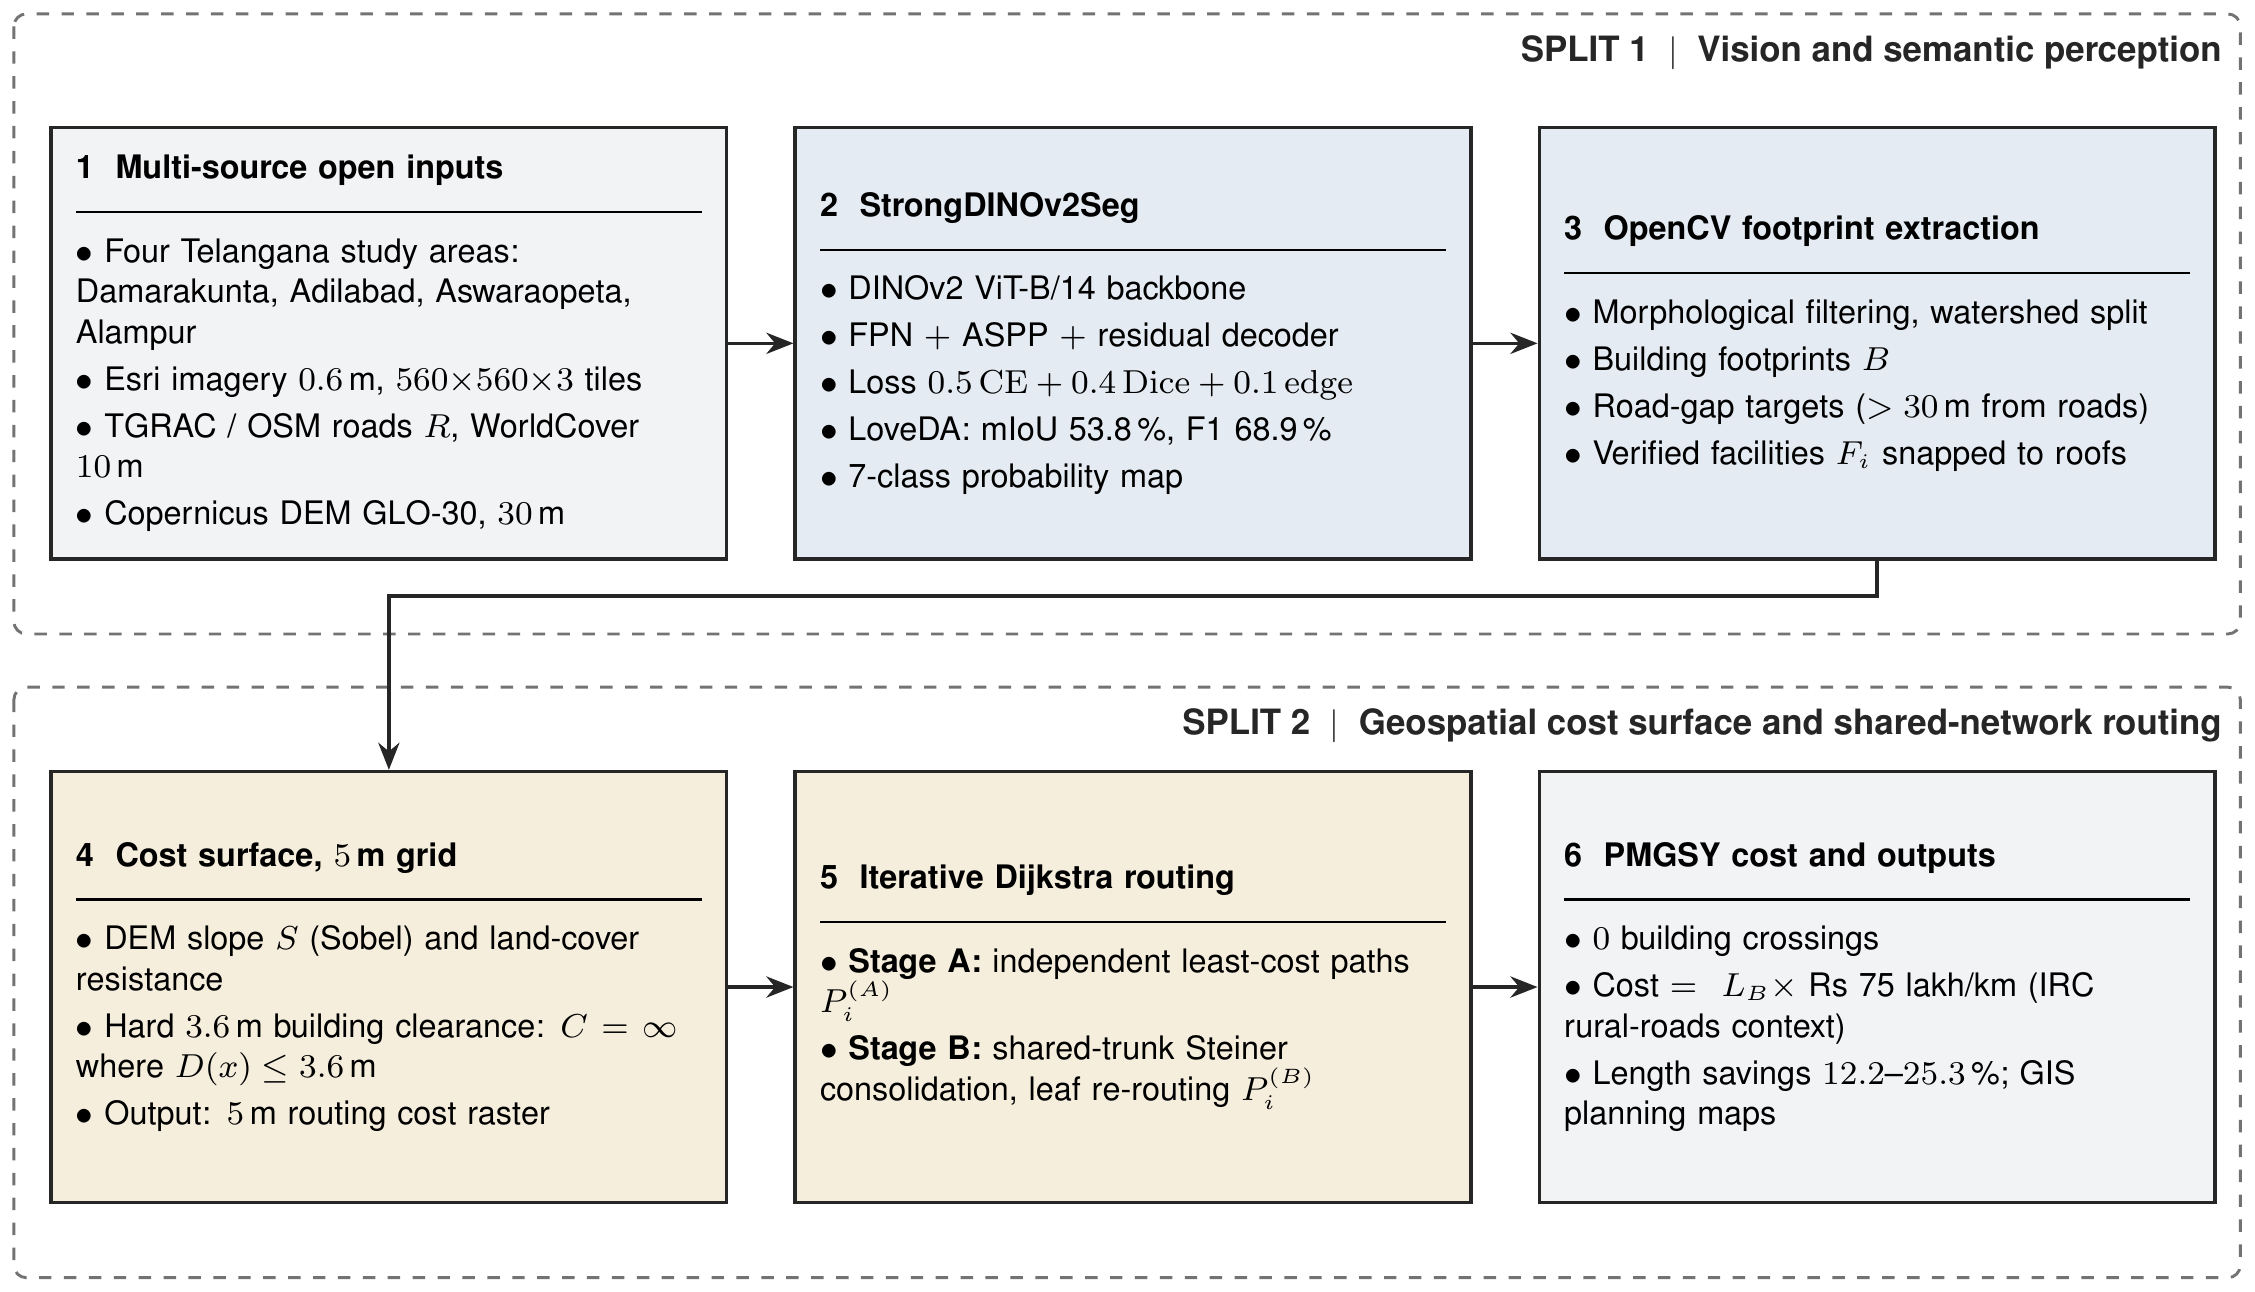
\includegraphics[width=\textwidth]{fig_architecture.png}
\caption{Two-split framework, applied unchanged to the four study areas. Split~1 (vision and semantic perception): (1)~multi-source open inputs (Esri World Imagery, roads from Overture and OSM, ESA WorldCover, Copernicus DEM, verified facilities $F_i$); (2)~\dinoseg{} semantic segmentation of $560\times560\times3$ RGB tiles (DINOv2 ViT-B/14: self-supervised vision transformer, base size, 14~px patches; FPN: feature pyramid network; ASPP: atrous spatial pyramid pooling; CE: cross-entropy; mIoU: mean intersection over union; F1: harmonic mean of precision and recall); (3)~OpenCV morphological and watershed footprint extraction with road-gap targets and facility snapping. Split~2 (geospatial cost surface and shared-network routing): (4)~$5$~m cost surface from DEM slope and land cover with a hard $3.6$~m building clearance; (5)~Stage~A independent and Stage~B shared-trunk Dijkstra routing; (6)~PMGSY-benchmarked cost, zero-crossing corridors and GIS planning maps (PMGSY: Pradhan Mantri Gram Sadak Yojana; IRC: Indian Roads Congress). AI-assisted workflow diagram: the framework diagram was drafted with a generative AI tool (Claude, Anthropic) and reviewed by the authors.}
\label{fig:arch}
\end{figure}

\begin{figure}[p]
\centering
\IfFileExists{fig_flow_study_areas.png}{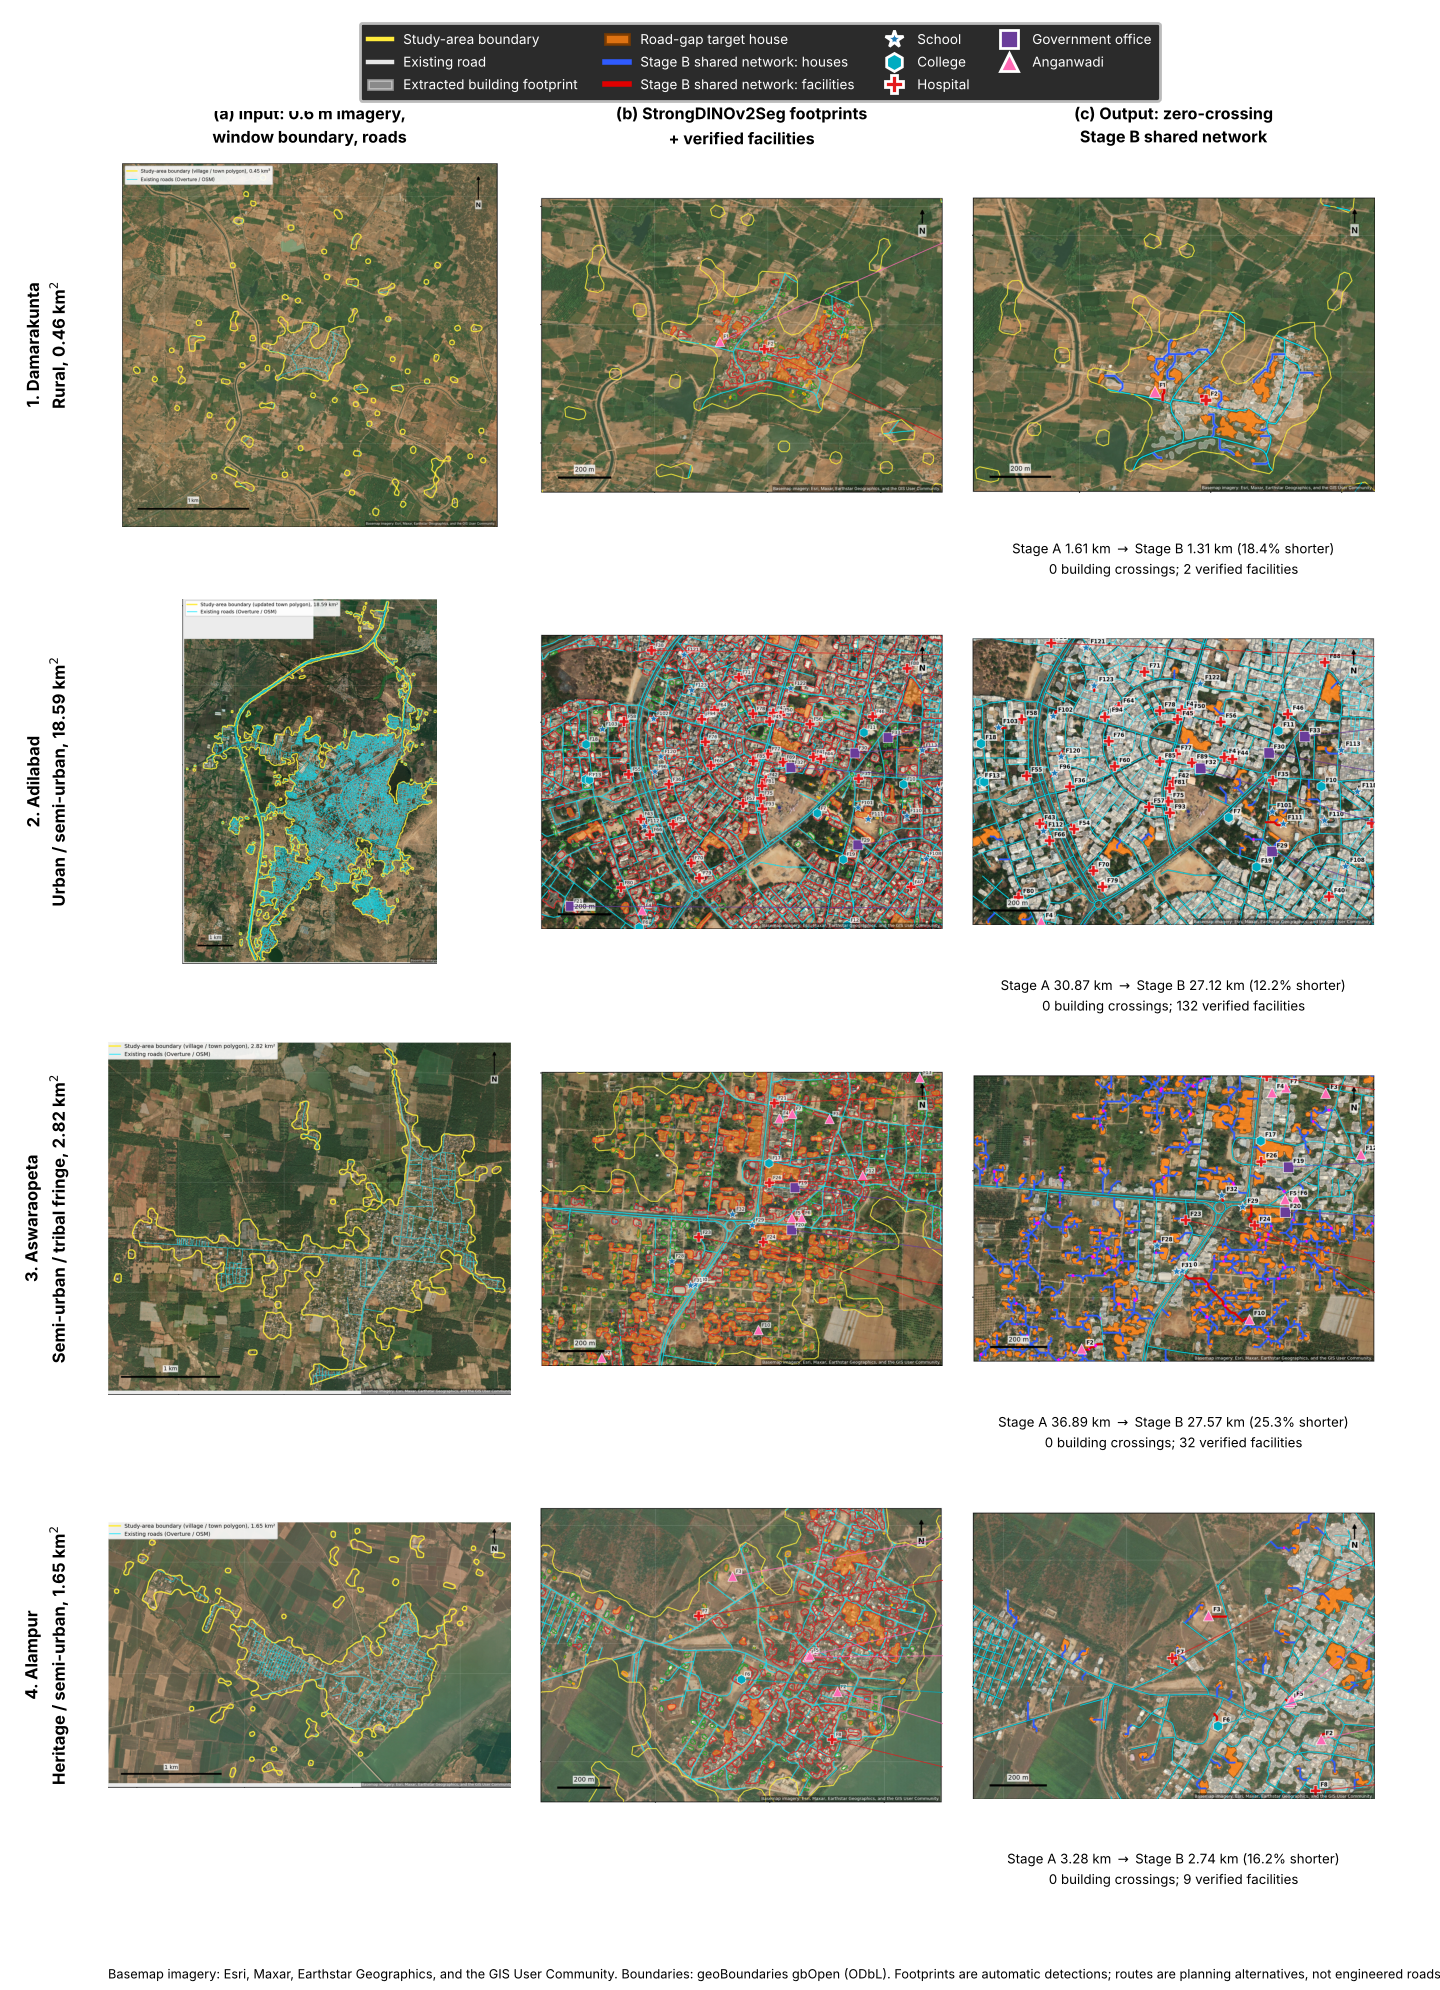
\includegraphics[width=\textwidth,height=0.68\textheight,keepaspectratio]{fig_flow_study_areas.png}}{\fbox{\parbox{0.8\textwidth}{\centering\pending{Figure not generated yet: run \texttt{python scripts/build\_paper\_flow\_figure.py --source segmentation}.}}}}
\caption{Study windows and end-to-end flow. Top: the key. One row per window, three columns: (a)~input (0.6~m Esri World Imagery, window boundary and existing roads); (b)~\dinoseg{} building footprints (road-gap target houses in orange) with the verified facilities; (c)~output, the Stage~B shared network of the 5~m zero-crossing plan (blue for houses, red for facilities) with scale bar and north arrow. Stage~A is the set of independent least-cost routes and Stage~B the shared network that consolidates them; below each output are their unique lengths, the building crossings and the facility count. Basemap imagery: Esri, Maxar, Earthstar Geographics, and the GIS User Community. Map lines delineate study areas and do not necessarily depict accepted national boundaries.}
\label{fig:flow}
\end{figure}


\subsubsection{Split 1: semantic segmentation with StrongDINOv2Seg}\label{sec:seg}
\dinoseg{} is a fully fine-tuned DINOv2 ViT-B/14 encoder \cite{oquab2023dinov2}, a vision transformer \cite{dosovitskiy2021vit}. Tokens from blocks 3, 6, 9 and 12 are projected to 256 channels and fused FPN-style \cite{lin2017fpn}, passed through an ASPP neck (rates 6, 12, 18) \cite{chen2018deeplabv3plus} and a four-stage decoder of residual convolution blocks \cite{he2016resnet} (256, 128, 64 and 32 channels) with auxiliary heads for deep supervision \cite{lee2015dsn}. \emph{Why LoveDA.} Telangana has no village-level pixel labels, and drawing them for every settlement would defeat the purpose of an open-data planning tool. LoveDA \cite{wang2021loveda} supplies standardised multi-class remote-sensing land-cover imagery, with urban and rural scenes and seven classes (background, building, road, water, barren, forest and agriculture), so it serves to pre-train and benchmark \dinoseg{} once; the frozen checkpoint is then applied to the open-data Telangana planning windows without any village-by-village labelling. Training used LoveDA at 560~px for a scheduled 10 epochs (AdamW \cite{loshchilov2019adamw}, cosine schedule \cite{loshchilov2017sgdr} to $10^{-7}$, encoder learning rate $\times 0.1$); the epoch-4 checkpoint is used for all four settlements, frozen, with SHA-256 \texttt{2e7c4646dc77ceb2\allowbreak a357f44f11cb3f7f\allowbreak f84e636871d70ba4\allowbreak c31e194e5ec00cf3}. With logits $\mathbf z$, labels $y$, class probabilities $p_{ic}$ and one-hot targets $t_{ic}$ at pixel $i$ (class 0 is ignored), the loss is
\begin{equation}
\begin{aligned}
\mathcal L(\mathbf z,y)&=0.5\,\mathcal L_{\mathrm{CE}}+0.4\,\mathcal L_{\mathrm{Dice}}+0.1\,\mathcal L_{\mathrm{edge}},\\
\mathcal L_{\mathrm{total}}&=\mathcal L(\mathbf z^{\mathrm{main}},y)+0.4\sum_{j=1}^{3}\mathcal L(\mathbf z^{(j)},y),
\end{aligned}
\label{eq:loss}
\end{equation}
\begin{equation}
\begin{aligned}
\mathcal L_{\mathrm{Dice}}&=\frac1{|\mathcal C|}\sum_{c\in\mathcal C}\Bigl(1-\frac{2\sum_i p_{ic}t_{ic}+\varepsilon}{\sum_i (p_{ic}+t_{ic})+\varepsilon}\Bigr),\\
\mathcal L_{\mathrm{edge}}&=\frac1{|\Omega|}\sum_{i\in\Omega}(1+4e_i)\,\mathrm{CE}_i,\\
e_i&=\min\{1,\,|(K_x{*}y)_i|+|(K_y{*}y)_i|\}.
\end{aligned}
\label{eq:diceedge}
\end{equation}
Here $\mathcal C$ is the set of scored classes, $\varepsilon$ a small smoothing constant, and $K_x,K_y$ the Sobel kernels, so that the edge term up-weights the cross-entropy of pixels on label boundaries by up to a factor of five \cite{milletari2016vnet}; the three auxiliary heads $\mathbf z^{(j)}$ provide deep supervision. From the confusion matrix, with $TP_c,FP_c,FN_c$ the true positives, false positives and false negatives of class $c$ and $N$ the number of labelled pixels,
\begin{equation}
\begin{aligned}
\mathrm{OA}&=\frac{\sum_c TP_c}{N},\qquad P_c=\frac{TP_c}{TP_c+FP_c},\\
R_c&=\frac{TP_c}{TP_c+FN_c},\qquad F_{1,c}=\frac{2P_cR_c}{P_c+R_c},\\
\mathrm{IoU}_c&=\frac{TP_c}{TP_c+FP_c+FN_c},
\end{aligned}
\label{eq:metrics}
\end{equation}
and $P$, $R$, $F_1$ (the Dice coefficient) and $\mathrm{mIoU}=|\mathcal C|^{-1}\sum_{c\in\mathcal C}\mathrm{IoU}_c$ are the macro averages over the scored classes (IoU as in \cite{everingham2010voc}); because $F_{1,c}$ equals the per-class Dice score, the reported F1-score is the mean Dice.

\subsubsection{Split 1: tiled inference, footprint extraction and road-gap targets}\label{sec:extract}
Each mosaic is segmented in $560\times560$~px tiles at a stride of 420~px with a 70~px margin discarded at inner tile edges (stride $\le$ tile $-\,2\times$ margin, so no gaps appear). Building instances are extracted from the predicted mask with OpenCV and NumPy \cite{bradski2000opencv,harris2020numpy} (algorithm~\ref{alg:extract}): a distance transform of each connected component \cite{felzenszwalb2012edt} gives $h$-maxima markers \cite{vincent1993morph}, a marker-controlled flooding of the inverted transform (a watershed-type split \cite{vincent1991watershed}) proposes pieces, and a neck test keeps two pieces apart only if the saddle between them is narrower than 0.65 times the inscribed radius of the smaller piece; otherwise they are re-merged. Blobs much larger than the median compact roof are flagged \textsc{Unresolved\_Merge} and treated as built-up extent rather than single houses. Because connecting every footprint is meaningless in a fabric already served by roads, only buildings more than 30~m (the planner snap distance) from an existing road are routed; planner cost grows roughly quadratically with the number of targets, which further motivates the filter.

\begin{algorithm}[t]
\footnotesize
\caption{Tiled \dinoseg{} inference and distance-transform building extraction (EDT: Euclidean distance transform; $h$-maxima: regional maxima of height $h$ used as seeds) (\texttt{run\_tiled\_inference.py}, \texttt{extract\_buildings\_v8.py})}
\label{alg:extract}
\begin{algorithmic}[1]
\Require mosaic $I$ (0.6~m), checkpoint $\theta$, tile $T=560$, stride $s=420$, margin $m=70$, neck ratio $\eta=0.65$, seed height $h=0.3$~m
\Ensure footprints $\mathcal B$ with quality classes
\State \textbf{assert} $s\le T-2m$ \Comment{no gaps between tile centres}
\For{each tile of size $T\times T$ at stride $s$}
  \State $p\gets\mathrm{softmax}(f_\theta(\text{tile}))$; write class $\arg\max p$ and $p_{\mathrm{bldg}}$ for the tile centre (drop $m$ px at inner edges)
\EndFor
\State $M\gets(\text{class}=\text{building})\wedge\lnot\text{no-data}$; drop components smaller than 6~m$^2$
\For{each connected component $K$ of $M$}
  \State $D\gets\mathrm{EDT}(K)$ (smoothed, $\sigma=1$ px); markers $\gets$ $h$-maxima of $D$ with height $h$
  \State pieces $\gets$ marker-controlled flooding of $-D$ (only if area $\ge 40$~m$^2$)
  \For{each adjacent piece pair $(a,b)$}
    \State $r_{ab}\gets D_{\mathrm{saddle}}/\min(D_a^{\max},D_b^{\max})$
    \If{$r_{ab}>\eta$ \textbf{or} a piece is smaller than 12~m$^2$} merge $a,b$ \Comment{no real neck}
    \EndIf
  \EndFor
\EndFor
\State polygonise; flag \textsc{Unresolved\_Merge} if area $>4\times$ the median compact roof; assign \textsc{Plausible} / \textsc{Review} / \textsc{Small} by confidence and shape
\State \Return $\mathcal B$
\end{algorithmic}
\end{algorithm}

\subsubsection{Split 1: facility audit and roof snapping}\label{sec:audit}
Overture Places alone mislocated or missed colleges, hospitals, offices and anganwadis, so the facilities of each area come from a four-pass audit (\texttt{scripts/audit\_facilities.py}). Pass~1 harvests candidates inside and within 500~m of the polygon from OpenStreetMap \cite{haklay2008osm} (Overpass and the Photon geocoder \cite{photon2026}), Overture Places, Wikidata and Wikipedia. Pass~2 assigns one of five categories (School, College, Hospital, Government Office, Anganwadi), removes closed or commercial records (pharmacies, laboratories, coaching centres, banks, cooperative societies), religious sites, foreign place names and placeholder coordinates shared by several differently named records, and merges duplicates of one campus across sources; every removal is logged with its reason. Pass~3 moves each survivor onto the footprint that contains it or, failing that, the nearest footprint of at least 25~m$^2$ within 35~m (a compound building up to 25~m away for a school, college or hospital), and removes facilities with no building in range. Pass~4 writes the verified table with the sources, the snap distance and a confidence label; records with a single source and a snap of more than 12~m are kept with \texttt{use\_in\_analysis}${}=$\,False and are not routed.

\subsubsection{Split 2: DEM slope, multi-criteria cost surface and building clearance}\label{sec:cost}
Let $\mathcal B$ be blocked cells (water, invalid cells, slope $>25^{\circ}$) and $\mathcal P$ the cells whose centre lies inside a footprint. The 10~m comparison graph has the unblocked cells as nodes and 8-neighbour edges with no diagonal corner-cutting, and the cell cost is
\begin{equation}
\begin{aligned}
c(x)&=\bigl[c_{\mathrm{lc}}(\ell(x))+g(S(x))\bigr]\,m(x),\\
m(x)&=\begin{cases}\mu & x\in\mathcal P\\ 1 & \text{otherwise,}\end{cases}
\end{aligned}
\label{eq:cell}
\end{equation}
where $\ell$ is the WorldCover class with resistance $c_{\mathrm{lc}}=8,5,3,6,2,4$ for trees, shrubland, grassland, cropland, built-up and bare/sparse land (classes 10, 20, 30, 40, 50, 60), $g(S)=w_s\min(S,S_{\mathrm{ref}})/S_{\mathrm{ref}}$ with $w_s=4$ and $S_{\mathrm{ref}}=10^{\circ}$, and $\mu=4$ is the soft footprint penalty. Slope comes from the Copernicus GLO-30 elevation $z$ with the Sobel gradient \cite{sobel1968gradient,horn1981hill} at the DEM spacing $\Delta_z=30$~m, resampled bilinearly to the planning grid:
\begin{equation}
\begin{aligned}
\partial_x z&\approx\frac{(K_x{*}z)}{8\Delta_z},\qquad \partial_y z\approx-\frac{(K_y{*}z)}{8\Delta_z},\\
S&=\arctan\sqrt{(\partial_x z)^2+(\partial_y z)^2},\qquad p_S=100\tan S,
\end{aligned}
\label{eq:slope}
\end{equation}
where $z$ is the elevation (m), $K_x$ and $K_y$ are the $3\times3$ Sobel kernels, $*$ is two-dimensional convolution, $\Delta_z=30$~m is the DEM grid spacing, $\partial_x z$ and $\partial_y z$ are the elevation gradients, $S$ is the slope in degrees (used in the cost surface) and $p_S$ the percentage slope reported in the tables; no separate IRC slope-penalty factor is applied. The soft penalty lets a route cross a roof when the detour costs more, so the proposed plan uses a hard barrier on a finer grid. Each 10~m cost cell is refined to $2\times2$ cells of size $\Delta=5$~m with the same cost per metre, and with $D(x)$ the Euclidean distance from the centre of cell $x$ to the nearest footprint (zero inside a footprint),
\begin{equation}
\begin{aligned}
C(x)&=c_{\mathrm{lc}}(\ell(x))+g(S(x))+C_{\mathrm{bldg}}(x),\\
C_{\mathrm{bldg}}(x)&=\begin{cases}\infty & D(x)\le r_c\\ 0 & \text{otherwise,}\end{cases}\\
r_c&=3.6\ \mathrm{m},\qquad \Delta=5\ \mathrm{m}.
\end{aligned}
\label{eq:bldg}
\end{equation}
Because $r_c>\Delta\sqrt2/2=3.54$~m, no step between two free cell centres can touch a footprint: a point of the step lies within $\Delta\sqrt2/2$ of one of its end points, and that end point would then have been blocked. A target sits inside its own building, so each route starts at the edge of that building and reaches the nearest free cell connected to the road network by a straight lane of at most the snap distance that touches no other footprint; a target with no such lane (a house enclosed by other buildings) is reported as unrouted, never routed over a roof. Lengths are measured from the building edge, and every drawn route (lane, path and road attachment) is finally intersected with all footprints other than its own.

\subsubsection{Split 2: shared-network routing by iterative Dijkstra search}\label{sec:routing}
The graph has the free cells as nodes and 8-neighbour edges, a diagonal step being allowed only if both orthogonal neighbours are free. The weight of an edge $(u,v)$ between neighbouring free cells $u$ and $v$, with $C(u)$ the cost of cell $u$ and $d(u,v)$ the step length, is
\begin{equation}
\begin{aligned}
w(u,v)&=d(u,v)\,\frac{C(u)+C(v)}{2},\\
d(u,v)&=\begin{cases}\Delta&\text{cardinal step}\\ \sqrt2\,\Delta&\text{diagonal step.}\end{cases}
\end{aligned}
\label{eq:edge}
\end{equation}
Stage~A gives every target $t$ the independent least-cost path $\pi_t^{A}=\arg\min_{\pi:\,t\to R}\sum_{e\in\pi}w(e)$ to the existing road cells $R$ \cite{dijkstra1959note,hart1968astar,collischonn2000lcp}, and two further alternatives that multiply $w(e)$ by $\lambda\in\{3,8\}$ on cells within 20~m of the earlier paths and overlap them by at most 80\% ($K=3$ alternatives in total). Stage~B starts from $E_S=\emptyset$ and repeatedly serves the target and route with the highest weight per marginal cost,
\begin{equation}
\begin{aligned}
(t^\star,\pi^\star)&=\arg\max_{t\in U,\ \pi\in\Pi_t\cup\{\pi_t^{\mathrm{net}}\}}\frac{\omega_t}{\Delta\Lcost(\pi\mid S)},\\
\Delta\Lcost(\pi\mid S)&=\sum_{e\in\pi\setminus E_S}w(e),
\end{aligned}
\label{eq:stageb}
\end{equation}
where $\omega_t$ weights the target (below), $E_S$ is the set of edges already built, $\Delta\Lcost(\pi\mid S)$ is the extra cost of route $\pi$ given the built network $S=E_S$, and $U$ is the set of unserved targets, $\Pi_t$ the Stage~A alternatives, $\pi_t^{\mathrm{net}}$ the least-cost path to the roads together with the routes already selected, and $\omega_t$ the priority weight (4 for hospitals and health centres, 3 for schools, colleges and anganwadis, 2 for government offices, 1 for houses). A built edge $e\in E_S$ costs nothing again---a discount factor $\alpha=0$ on $E_S$---so a route may end on another route; this is the shortest-path heuristic for Steiner trees \cite{kou1981steiner,mehlhorn1988steiner} on a penalised, land-cover-weighted graph with the road network as a free sub-tree, and it carries no optimality guarantee. Two passes of leaf re-routing follow. Snap distance is 30~m, search limit 1{,}500~m and attachment tolerance 15~m; facilities are planned in a separate phase.

\begin{algorithm}[t]
\footnotesize
\caption{Cost surface with zero-crossing clearance and two-stage routing (\texttt{clearance.py}, \texttt{plan\_network\_v2.py})}
\label{alg:route}
\begin{algorithmic}[1]
\Require land cover $\ell$, DEM $z$, roads $R$, footprints $\mathcal B$, targets $\mathcal T$ (road-gap houses and verified facilities with weights $\omega_t$), $\Delta=5$~m, $r_c=3.6$~m, $K=3$
\Ensure route sets $\{\pi_t^A\}$, $E_S$ and lengths $L_A$, $L_B$, saving $\rho$, cost
\State $S\gets$ slope of $z$ (equation~\ref{eq:slope}); $C_0(x)\gets c_{\mathrm{lc}}(\ell(x))+g(S(x))$; block water, invalid cells and $S>25^{\circ}$
\State refine $C_0$ from 10~m to $\Delta=5$~m (same cost per metre); $D\gets\mathrm{EDT}(\mathcal B)$; $C(x)\gets\infty$ where $D(x)\le r_c$
\State keep the free cells connected to a road cell; edge weights $w$ by equation~\ref{eq:edge}
\For{each target $t\in\mathcal T$}
  \State entrance $e_t\gets$ point of the target's building edge nearest to a free cell $s_t$; require a lane $e_t\to s_t$ of at most 30~m that touches no other footprint, else mark $t$ unrouted
  \State $\Pi_t\gets K$ Dijkstra alternatives from $s_t$ to $R$ (corridor inflation $\lambda\in\{3,8\}$, 20~m, overlap $\le 80\%$); $\pi_t^A\gets$ first alternative
\EndFor
\State $L_A\gets L(\{\pi_t^A\})$; $U\gets$ routed targets; $E_S\gets\emptyset$
\While{$U\ne\emptyset$}
  \For{each $t\in U$} add the least-cost path $\pi_t^{\mathrm{net}}$ to $R\cup E_S$ to the candidates $\Pi_t$ \EndFor
  \State $(t^\star,\pi^\star)\gets\arg\max\ \omega_t/\Delta\Lcost(\pi\mid S)$ (equation~\ref{eq:stageb}); $E_S\gets E_S\cup\pi^\star$; $U\gets U\setminus\{t^\star\}$
\EndWhile
\State two leaf re-route passes: replace a route that no other route uses if it has become cheaper given the others
\State verify $X=0$ (equation~\ref{eq:saving}); $L_B\gets L(E_S)$; $\rho\gets 100(L_A-L_B)/L_A$; cost by equation~\ref{eq:cost}
\end{algorithmic}
\end{algorithm}

\subsubsection{Split 2: network metrics and PMGSY cost estimation}\label{sec:eval}
With $L(\cdot)$ the total length of the unique edges of a route set (shared edges counted once), the saving of the shared network and the exposure of dwellings are
\begin{equation}
\begin{aligned}
\rho&=\frac{L_A-L_B}{L_A}\times100\%,\\
L_A&=L\bigl(\{\pi_t^A\}\bigr),\qquad L_B=L(E_S),\\
X&=\sum_{r}\Bigl|r\cap\bigcup_{b\ne b_r}b\Bigr|=0.
\end{aligned}
\label{eq:saving}
\end{equation}
where $X$ is the length of routes inside footprints other than the route's own building $b_r$ (zero by construction under equation~\ref{eq:bldg}). The corridor cost is benchmarked against the PMGSY programme \cite{pmgsy}:
\begin{equation}
\begin{aligned}
\mathrm{Cost}_{\mathrm{INR\ lakh}}&=L_B[\mathrm{km}]\times c_{\mathrm{PMGSY}},\\
c_{\mathrm{PMGSY}}&=75\ \text{lakh/km}\ (\text{sensitivity range }60\text{--}90),
\end{aligned}
\label{eq:cost}
\end{equation}
where $L_B$ is the unique Stage~B length in kilometres, $c_{\mathrm{PMGSY}}$ the benchmark cost per kilometre and 1 lakh $=10^{5}$~INR (Indian rupees). This unit rate is the single benchmark used throughout for the unique shared corridor; it excludes land, drainage structures and variation in cross-section (design practice for the programme is set out in the Indian Roads Congress (IRC) rural roads manual \cite{irc2002sp20}), and its scope is stated in section~\ref{sec:disc}. Four strategies are compared on the 10~m soft-penalty grid in all four windows: straight lines, independent least-cost routes, a length-only control (cost surface replaced by distance), a roads-only shared reference (routes may share edges only with the existing road network) and the two-stage shared plan. The exposure metrics are the number of routes crossing another house's footprint and the route length inside other footprints.


\FloatBarrier
\section{Results}\label{sec:results}
\subsection{Land-cover segmentation and building footprint accuracy}\label{sec:res1}
On the 1{,}669-image LoveDA validation split (560~px tiles, seven scored classes) the epoch-4 checkpoint reached 53.8\% mIoU, 68.9\% Dice (equal to the macro F1-score), 71.3\% pixel accuracy, 72.4\% macro precision and 66.9\% macro recall; for the Building class IoU is 54.0\%, Dice 70.1\%, precision 62.1\% and recall 80.6\% (table~\ref{tab:seg}). The high building recall is what the routing task needs, because a missed roof removes a household from the plan whereas a spurious blob is absorbed by the merge flag and the 25~m$^2$ minimum. The published test-set mIoU of other LoveDA baselines are listed for orientation; they were scored on the benchmark's test split with other protocols, so the comparison is indicative. The scores are source-domain figures: no surveyed building mask exists for any Telangana window, so the footprints are described by their quality classes (figure~\ref{fig:split1}). Plausible single roofs make up 46\%, 46\%, 62\% and 52\% of the instances in Damarakunta, Adilabad, Aswaraopeta and Alampur, and merged roof blocks 42\%, 51\%, 36\% and 41\%, rising with the density of the fabric; the targets of the dense windows are therefore built-up units rather than individual houses.

\begin{table}[t]
\caption{Semantic segmentation on LoveDA. mIoU is the mean intersection over union over classes, F1 is the harmonic mean of precision and recall (equal to the Dice coefficient), and precision and recall are the share of predicted pixels that are correct and of true pixels that are found. (a)~Published mIoU of the benchmark baselines (test split, from the cited papers) next to \dinoseg{} (our 1{,}669-image validation split, so the comparison is indicative). (b)~Validation metrics of \dinoseg{} at 560~px: macro averages over the seven scored classes and the Building class alone. Overall pixel accuracy, a whole-image quantity with no per-class counterpart, is 71.3\%.}
\label{tab:seg}
\centering
\scriptsize
\setlength{\tabcolsep}{3pt}
\begin{minipage}[t]{0.47\textwidth}\centering
\begin{adjustbox}{max width=\textwidth}
\begin{tabular}{@{}llr@{}}
\toprule
\multicolumn{3}{@{}l}{\textit{(a) Literature comparison on LoveDA}}\\
Model & Backbone & Published mIoU (\%)\\
\midrule
U-Net \cite{ronneberger2015unet,wang2021loveda} & ResNet-50 & 47.84\\
DeepLabv3+ \cite{chen2018deeplabv3plus,wang2021loveda} & ResNet-50 & 47.62\\
UNetFormer \cite{wang2022unetformer} & ResNet-18 & 52.4\\
\dinoseg{} (ours) & DINOv2 ViT-B/14 & 53.8\\
\bottomrule
\end{tabular}
\end{adjustbox}
\end{minipage}\hfill
\begin{minipage}[t]{0.5\textwidth}\centering
\begin{adjustbox}{max width=\textwidth}
\begin{tabular}{@{}lrrrr@{}}
\toprule
\multicolumn{5}{@{}l}{\textit{(b) \dinoseg{} validation metrics (560 px, 1,669 images)}}\\
Scope & mIoU (\%) & F1 / Dice (\%) & Precision (\%) & Recall (\%)\\
\midrule
All 7 classes (macro) & 53.8 & 68.9 & 72.4 & 66.9\\
Building class & 54.0 & 70.1 & 62.1 & 80.6\\
\bottomrule
\end{tabular}
\end{adjustbox}
\end{minipage}
\end{table}

\begin{figure}[!t]
\centering
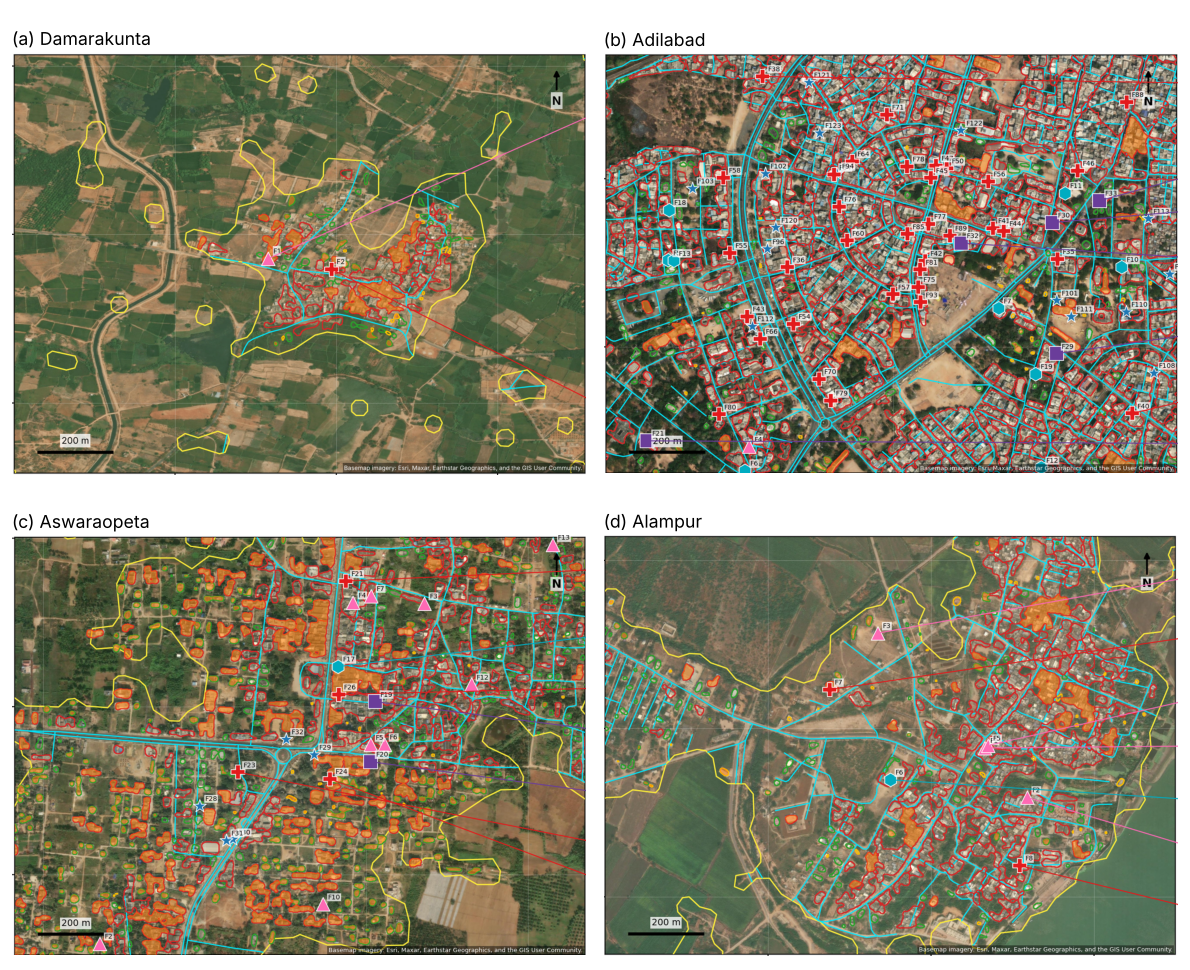
\includegraphics[width=\textwidth,height=0.42\textheight,keepaspectratio]{fig_split1_footprints.png}
\caption{Split~1 output in the densest cluster of each study window: building footprints extracted by \dinoseg{} and OpenCV (orange: road-gap target houses; outlined: other footprints), verified public facilities (School, College, Hospital, Government Office, Anganwadi, with their facility numbers) and existing roads (cyan). Scale bars are 200~m. Basemap imagery: Esri, Maxar, Earthstar Geographics, and the GIS User Community. Map lines delineate study areas and do not necessarily depict accepted national boundaries.}
\label{fig:split1}
\end{figure}


\subsection{Multi-criteria cost surfaces and proposed road connectivity across the four study windows}\label{sec:res2}
The cost surface adds a land-cover resistance and a slope penalty to a hard building clearance (equations~\ref{eq:cell}--\ref{eq:bldg}); the terrain is nearly flat in all four windows, with mean slopes of 3.8, 3.1, 3.1 and 2.1\% (figure~\ref{fig:cost}), so cost differences come mainly from land cover and from the blocked cells around buildings. On the $5$~m grid with the $3.6$~m clearance every window yields a connected plan with no route across a roof (table~\ref{tab:four}). In Damarakunta, 27 of 27 road-gap targets are routed and 2 verified facilities are connected; in Adilabad 607 of 613 targets and 132 facilities; in Aswaraopeta 632 of 678 targets and 32 facilities; and in Alampur 58 of 59 targets and 9 facilities. The few unrouted targets are houses enclosed by neighbouring buildings and are reported as unrouted rather than routed over a roof. A $10$~m cell is wider than the lanes between neighbouring buildings, so a coarse grid with only a soft footprint penalty cannot keep routes off roofs, whereas a $5$~m grid that blocks every cell within $3.6$~m of a footprint (above the $3.54$~m half-diagonal of a $5$~m cell) leaves no step that can touch a roof; every drawn route was checked against all other footprints.

\begin{figure}[!t]
\centering
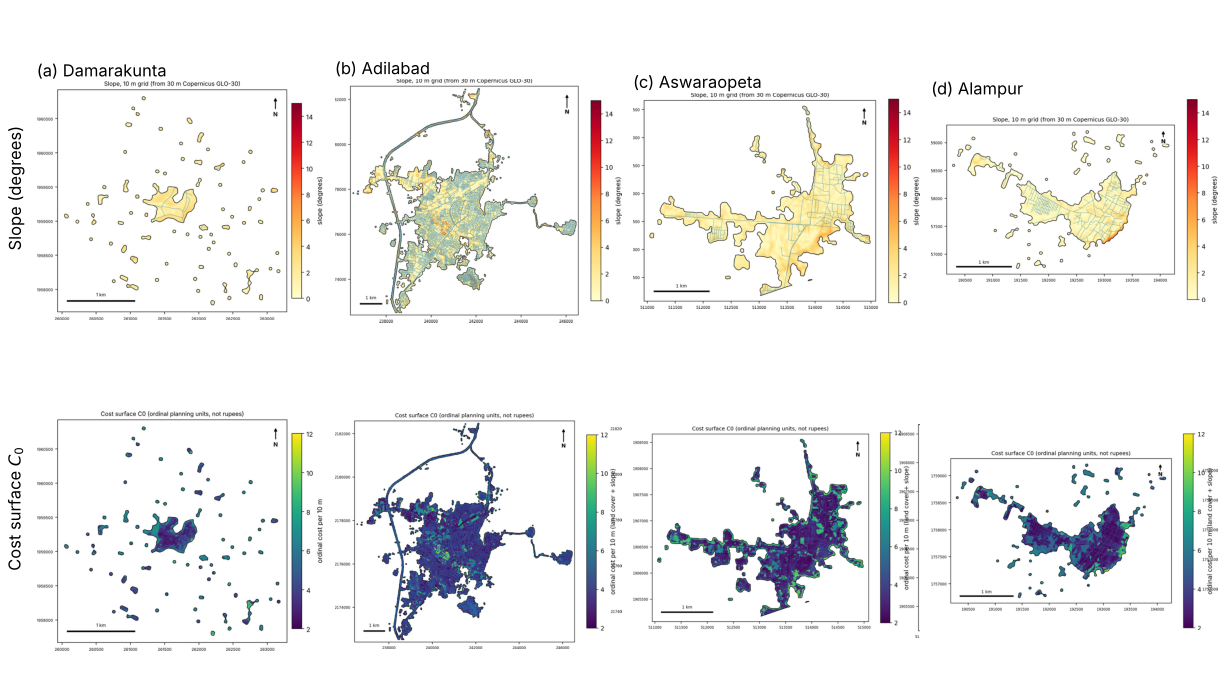
\includegraphics[width=\textwidth,height=0.36\textheight,keepaspectratio]{fig_split2_cost_surface.png}
\caption{Split~2 inputs for the four study windows. Top: terrain slope in degrees from the 30~m Copernicus GLO-30 DEM (digital elevation model), resampled to the 10~m planning grid. Bottom: the base cost surface $C_0$ in ordinal planning units per 10~m, the sum of the land-cover resistance and the slope penalty (equation~\ref{eq:cell}); cells that are water, invalid or steeper than 25$^{\circ}$ are blocked. Map lines delineate study areas and do not necessarily depict accepted national boundaries.}
\label{fig:cost}
\end{figure}


\begin{table}[t]
\caption{Four study windows side by side. Segmentation rows: LoveDA validation of the single \dinoseg{} checkpoint (overall accuracy is the share of correctly classified pixels; precision and recall are macro averages over classes; F1-score equals the mean Dice coefficient; mIoU is the mean intersection over union). Stage~A is independent least-cost routing and Stage~B the shared-trunk network; PMGSY is the Pradhan Mantri Gram Sadak Yojana rural road programme; 1 lakh $=10^{5}$ INR (Indian rupees); slope is the mean terrain slope in percent. Routing rows: unique lengths on the 5~m zero-crossing grid (shared edges once); building crossings are routes inside another building's footprint; cost is the Stage~B length times Rs 75 lakh per km (range 60--90).}
\label{tab:four}
\centering
\scriptsize
\resizebox{\textwidth}{!}{% generated by scripts/run_village_pipeline.py --compare-all (do not edit by hand); \pending{...} marks a value not yet computed on the machine that generated this file
\begin{tabular}{@{}lrrrr@{}}
\toprule
Metric & Damarakunta & Adilabad & Aswaraopeta & Alampur \\
\midrule
\multicolumn{5}{@{}l}{\textit{Study area profile}}\\
District & Siddipet & Adilabad & Bhadradri Kothagudem & Jogulamba Gadwal \\
Typology & Rural & Urban / semi-urban & Semi-urban / tribal fringe & Heritage / semi-urban \\
Window area (km$^2$) & 0.46 & 18.59 & 2.82 & 1.65 \\
Existing road length (km) & 3.5 & 509.9 & 28.6 & 25.3 \\
\midrule
\multicolumn{5}{@{}l}{\textit{Segmentation and extraction (model metrics: LoveDA validation, one checkpoint for all areas)}}\\
Overall accuracy (\%) & \multicolumn{4}{c}{71.3} \\
Precision, macro (\%) & \multicolumn{4}{c}{72.4} \\
Recall, macro (\%) & \multicolumn{4}{c}{66.9} \\
F1-score = mean Dice (\%) & \multicolumn{4}{c}{68.9} \\
mIoU (\%) & \multicolumn{4}{c}{53.8} \\
Extracted building footprints & 100 & 5{,}653 & 1{,}297 & 430 \\
\midrule
\multicolumn{5}{@{}l}{\textit{Verified public infrastructure (audited, on building footprints)}}\\
School & 0 & 39 & 5 & 1 \\
College & 0 & 15 & 3 & 1 \\
Hospital & 1 & 59 & 7 & 2 \\
Government office & 0 & 15 & 3 & 0 \\
Anganwadi & 1 & 4 & 14 & 5 \\
Total verified facilities & 2 & 132 & 32 & 9 \\
\midrule
\multicolumn{5}{@{}l}{\textit{Stage A vs.\ Stage B routing (5\,m zero-crossing clearance) and PMGSY-benchmarked cost}}\\
Road-gap target buildings & 27 & 613 & 678 & 59 \\
Routed buildings & 27 & 607 & 632 & 58 \\
Stage A independent length (km) & 1.61 & 30.87 & 36.89 & 3.28 \\
Stage B shared-trunk length (km) & 1.31 & 27.12 & 27.57 & 2.74 \\
Corridor length saving (\%) & 18.4 & 12.2 & 25.3 & 16.2 \\
Building crossings (routes) & 0 & 0 & 0 & 0 \\
Mean terrain slope (\%) & 3.8 & 3.1 & 3.1 & 2.1 \\
PMGSY-benchmarked cost (INR lakh) & 98 & 2{,}034 & 2{,}067 & 206 \\
\bottomrule
\end{tabular}
% PMGSY-benchmarked cost = unique Stage B length (km) x Rs 75 lakh/km (sensitivity range 60-90)
}
\end{table}

\subsection{Stage A versus Stage B and shared-network routing trade-offs}\label{sec:res3}
Consolidating the independent routes into a shared trunk shortens the unique network in every window (figure~\ref{fig:ab}): Stage~A needs 1.61, 30.87, 36.89 and 3.28~km and Stage~B 1.31, 27.12, 27.57 and 2.74~km in Damarakunta, Adilabad, Aswaraopeta and Alampur, savings of 18.4\%, 12.2\%, 25.3\% and 16.2\%, or Rs 98, 2{,}034, 2{,}067 and 206 lakh at the PMGSY benchmark. The saving is largest where targets are numerous, clustered and far from the mapped roads (Aswaraopeta) and smallest where the dense road layer already serves most houses and the remaining targets are scattered (Adilabad). Unique length scales with the number of targets and the road coverage, not with the window size: Aswaraopeta needs almost as much new road as Adilabad (27.57~km against 27.12~km) from one-seventh of the area. Figure~\ref{fig:detail} shows the shared trunks at settlement scale.

Table~\ref{tab:strategies} sets the two-stage plan against three baselines on the $10$~m soft-penalty grid, with the same targets and cost surface in each window. The two-stage plan is the shortest in all four windows (10.9\%, 14.4\%, 31.2\%, 17.8\% below independent routes); the roads-only shared reference recovers 0.1\%, 3.2\%, 1.7\%, 4.9\% and the length-only control 15.5\% shorter, 6.8\% shorter, 16.5\% longer, 8.2\% shorter, so sharing among the new routes, not sharing with existing roads or merely minimising length, drives the gain.

\begin{figure}[!t]
\centering
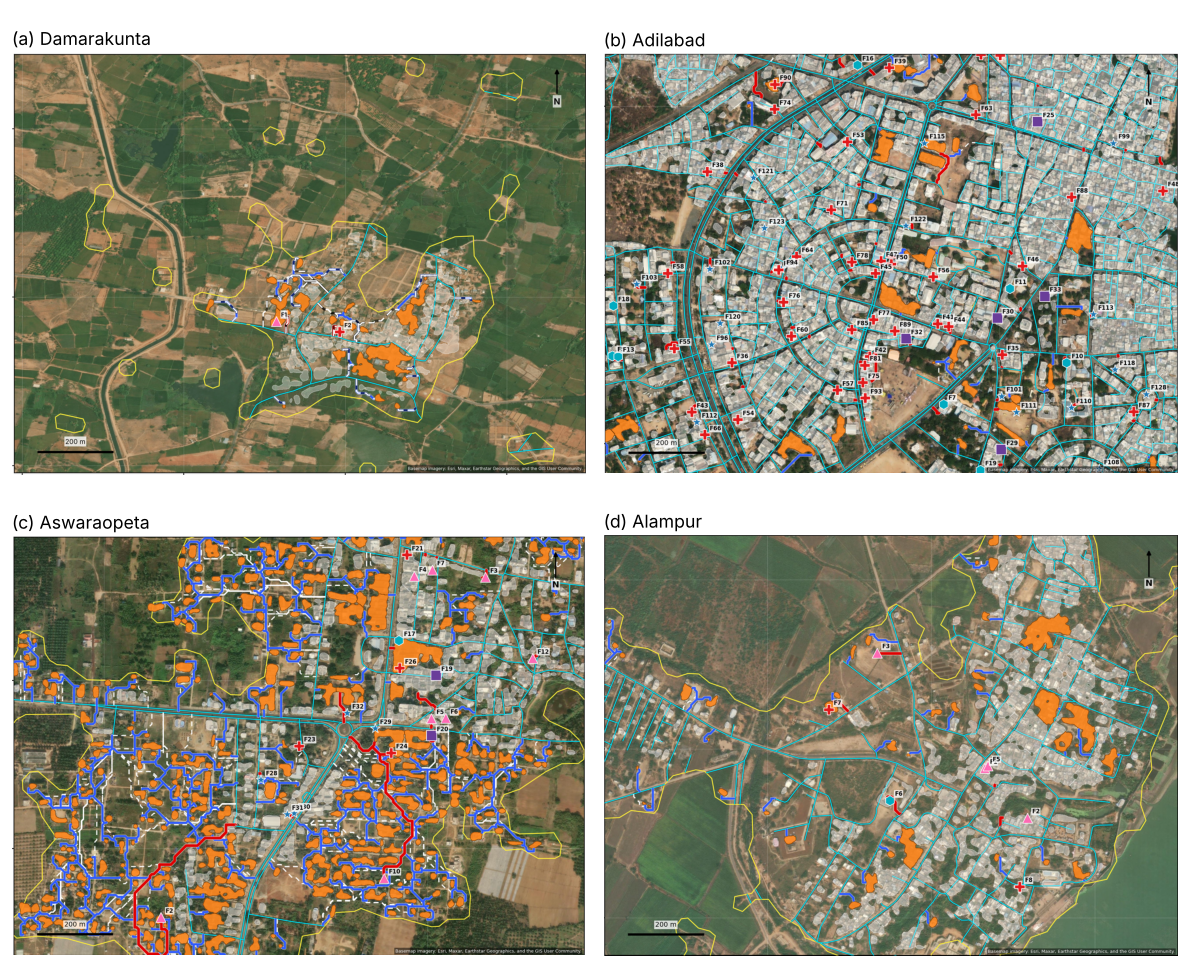
\includegraphics[width=\textwidth,height=0.42\textheight,keepaspectratio]{fig_stage_AB.png}
\caption{Stage~A against Stage~B in the densest cluster of each window: the white dashed lines are the independent least-cost routes (Stage~A first choice), the blue lines the shared network for houses and the red lines the shared network for facilities (Stage~B), on the $5$~m grid with the $3.6$~m building clearance. Orange footprints are road-gap target houses. Basemap imagery: Esri, Maxar, Earthstar Geographics, and the GIS User Community. Map lines delineate study areas and do not necessarily depict accepted national boundaries.}
\label{fig:ab}
\end{figure}

\begin{figure}[!t]
\centering
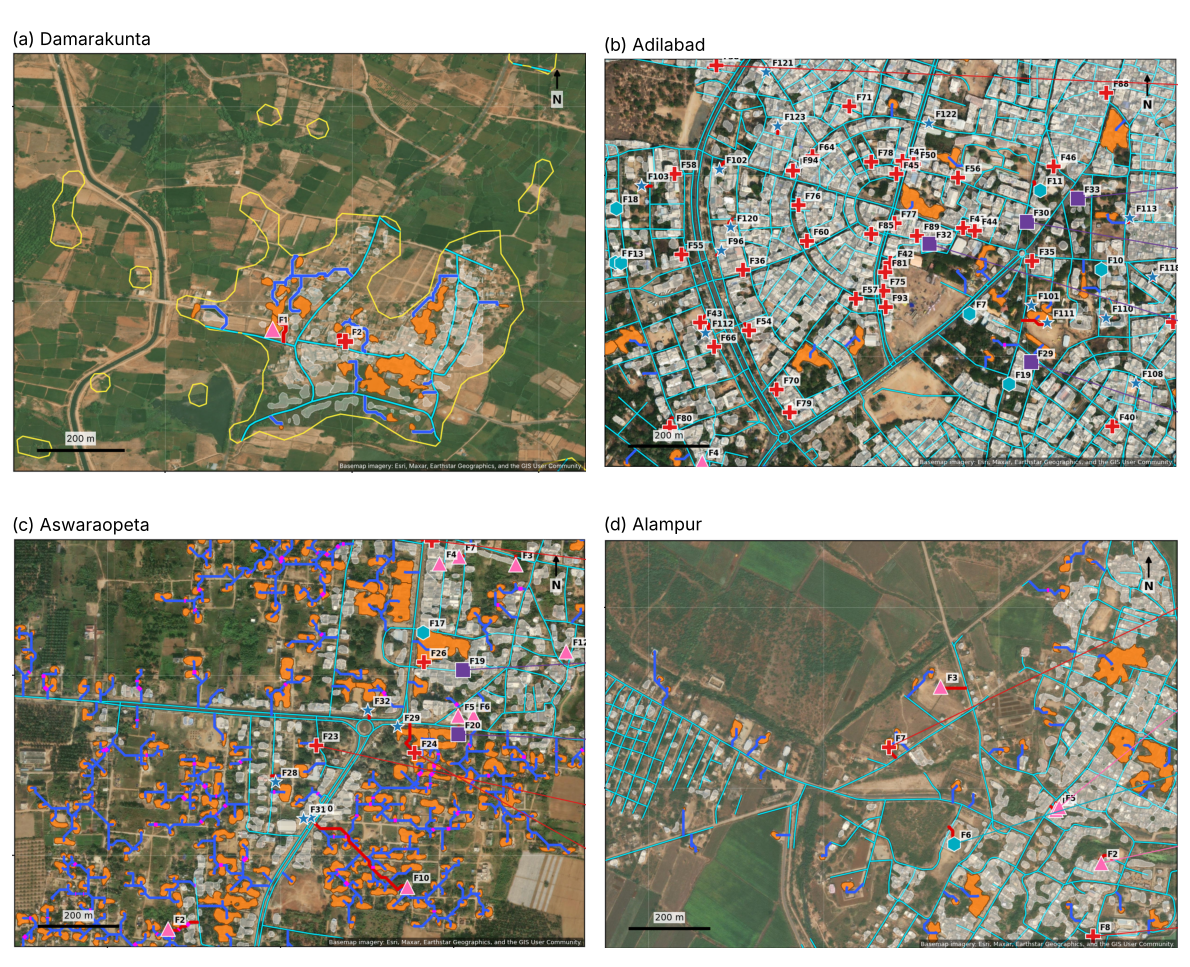
\includegraphics[width=\textwidth,height=0.42\textheight,keepaspectratio]{fig_shared_network_detail.png}
\caption{Settlement-scale detail of the zero-crossing shared network in each window (same window as the master planning map): house routes in blue, facility routes in red, verified facilities with their numbers, existing roads in cyan. No route crosses a building footprint. Basemap imagery: Esri, Maxar, Earthstar Geographics, and the GIS User Community. Map lines delineate study areas and do not necessarily depict accepted national boundaries.}
\label{fig:detail}
\end{figure}


\begin{table}[t]
\caption{Routing strategies on the $10$~m soft-penalty grid in the four study windows. Unique length counts shared edges once; saving is against independent routes (negative: longer); routes crossing is the number of routes that cross another building's footprint, and the last column is their length inside footprints. The length-only control replaces the cost surface by distance; the roads-only shared reference lets routes share edges only with the existing roads; the two-stage plan is the shared network of section~\ref{sec:routing}.}
\label{tab:strategies}
\centering
\scriptsize
\begin{adjustbox}{max width=\textwidth}
\begin{tabular}{@{}llrrrrr@{}}
\toprule
Window & Strategy & Routed & Unique length (m) & Saving (\%) & Routes crossing & In footprints (m)\\
\midrule
Damarakunta & Independent routes & 27 & 1{,}654.3 & 0.0 & 6 & 69.0\\
& Length-only control & 27 & 1{,}398.5 & 15.5 & 15 & 317.8\\
& Roads-only shared reference & 27 & 1{,}652.4 & 0.1 & 6 & 69.0\\
& Two-stage shared plan & 27 & 1{,}473.2 & 10.9 & 7 & 48.0\\
\midrule
Adilabad & Independent routes & 607 & 36{,}254.0 & 0.0 & 83 & 649.0\\
& Length-only control & 607 & 33{,}792.8 & 6.8 & 154 & 2{,}639.6\\
& Roads-only shared reference & 607 & 35{,}076.8 & 3.2 & 89 & 767.7\\
& Two-stage shared plan & 607 & 31{,}048.2 & 14.4 & 99 & 677.0\\
\midrule
Aswaraopeta & Independent routes & 636 & 43{,}136.5 & 0.0 & 286 & 3{,}249.5\\
& Length-only control & 636 & 50{,}265.1 & $-16.5$ & 446 & 17{,}593.7\\
& Roads-only shared reference & 636 & 42{,}391.4 & 1.7 & 320 & 4{,}927.3\\
& Two-stage shared plan & 636 & 29{,}657.6 & 31.2 & 157 & 1{,}090.4\\
\midrule
Alampur & Independent routes & 58 & 4{,}056.9 & 0.0 & 7 & 58.0\\
& Length-only control & 58 & 3{,}723.6 & 8.2 & 14 & 726.6\\
& Roads-only shared reference & 58 & 3{,}856.5 & 4.9 & 9 & 39.5\\
& Two-stage shared plan & 58 & 3{,}334.6 & 17.8 & 5 & 32.9\\
\bottomrule
\end{tabular}
\end{adjustbox}
\end{table}


\subsection{Cross-source footprint agreement, graph baselines, accessibility and error propagation}\label{sec:res4}
Four automated checks extend the main comparison. They use only the open layers of the Data section, no manual labelling and no field survey, and they are run by \texttt{footprint\_crossval.py}, \texttt{steiner\_baseline.py}, \texttt{accessibility\_metrics.py} and \texttt{aggregate\_sweeps.py}; their outputs are in \path{DELIVERABLES_CONTRIBUTION_3_MULTI_VILLAGE/validation}. They therefore measure agreement between open datasets and planning behaviour, not accuracy against ground truth.

\textbf{Cross-source footprint agreement.} Table~\ref{tab:xval} compares the segmentation footprints with Overture Maps buildings (OpenStreetMap and Google Open Buildings sources, release 2026-10-21.0) and, in Damarakunta, with the raw Google Open Buildings v3 polygons, inside each window's model-coverage region (the window intersected with the 30~m-buffered convex hull of the footprints; for Damarakunta this is 0.244 of 0.455~km$^2$ because the stored footprints cover part of the window only, and over the whole window the detection recall is 0.430 instead of 0.547). Against all Overture sources, area IoU is 0.283--0.373, area precision (share of our area covered by the reference) 0.371--0.437 and area recall (share of the reference area covered by our footprints) 0.495--0.717 across the four windows. At the object level, detection precision (share of our footprints that touch a reference building) is 0.893--0.950 and detection recall (share of reference buildings whose representative point lies in one of our footprints) is 0.515--0.747. Between 40 and 52\% of our footprints contain two or more Overture buildings: the model groups dense contiguous roofs, so one-to-one instance matching at IoU~0.5 reaches an F1 of only 0.010--0.022 and is not a meaningful score for these footprints. The agreement differs by source: the human-mapped OpenStreetMap subset is covered far more completely than the machine-derived Google subset in Adilabad (detection recall 0.860 against 0.554) and in Alampur (0.791 against 0.332), whereas its subset has only 7 features in Aswaraopeta and too few to score (fewer than five) in Damarakunta, and is not tabulated for either. No reference is treated as truth, since each has its own omissions and merging. Most of our footprints touch an open-inventory building, but our footprints reach only about half to three quarters of the reference buildings and group dense roofs, which is the footprint-granularity limitation that the error-propagation test below quantifies.

\begin{table}[t]
\caption{Agreement of the segmentation footprints with open building inventories inside each window's model-coverage region. Area P is the share of our footprint area covered by the reference, area R the share of the reference area covered by our footprints; detection P is the share of our footprints that touch a reference building, detection R the share of reference buildings whose representative point lies in one of our footprints; merged is the share of our footprints that contain two or more Overture buildings. Sub-source rows with fewer than 100 reference features are not shown. These are agreement figures between open datasets, not accuracy against ground truth.}
\label{tab:xval}
\centering
\footnotesize
\begin{adjustbox}{max width=\textwidth}
\begin{tabular}{@{}llrrrrrrr@{}}
\toprule
Window & Reference & Ref.\ $n$ & Area IoU & Area P & Area R & Detect.\ P & Detect.\ R & Merged (\%)\\
\midrule
Damarakunta & Overture, all sources & 578 & 0.299 & 0.382 & 0.579 & 0.950 & 0.547 & 46.0\\
 & Overture, Google subset & 577 & 0.299 & 0.382 & 0.580 & 0.950 & 0.548 & 46.0\\
 & Google Open Buildings v3 (raw) & 787 & 0.347 & 0.465 & 0.577 & 0.970 & 0.551 & 59.0\\
\addlinespace
Adilabad & Overture, all sources & 38{,}296 & 0.373 & 0.437 & 0.717 & 0.918 & 0.747 & 52.0\\
 & Overture, OSM subset & 24{,}178 & 0.285 & 0.308 & 0.791 & 0.515 & 0.860 & 32.9\\
 & Overture, Google subset & 14{,}118 & 0.118 & 0.129 & 0.586 & 0.615 & 0.554 & 23.2\\
\addlinespace
Aswaraopeta & Overture, all sources & 4{,}749 & 0.302 & 0.436 & 0.495 & 0.935 & 0.515 & 40.2\\
 & Overture, Google subset & 4{,}742 & 0.319 & 0.434 & 0.546 & 0.934 & 0.515 & 40.2\\
\addlinespace
Alampur & Overture, all sources & 3{,}343 & 0.283 & 0.371 & 0.546 & 0.893 & 0.565 & 44.0\\
 & Overture, OSM subset & 1{,}693 & 0.222 & 0.242 & 0.729 & 0.560 & 0.791 & 30.2\\
 & Overture, Google subset & 1{,}650 & 0.106 & 0.129 & 0.371 & 0.667 & 0.332 & 24.7\\
\bottomrule
\end{tabular}
\end{adjustbox}
\end{table}

\textbf{Graph-routing baselines.} Table~\ref{tab:graphbase} sets Stage~A and Stage~B against two classical baselines on the planner's own graph: the $5$~m clearance grid, the same cost surface and edge weights, the hard $3.6$~m building clearance and the existing-road cells as goals. The Kou--Markowsky--Berman Steiner tree \cite{kou1981steiner} (metric closure of the road network and the targets, minimum spanning tree, shortest-path expansion, second spanning tree and leaf pruning) is the standard 2-approximation for the same problem; the Euclidean minimum spanning tree joins the targets and the nearest road by straight lines. The comparison uses the house targets that Stage~B routed and counts unique grid-edge length without the short per-route connectors, so its lengths are slightly below the Stage~A and Stage~B lengths of the main results, which include the connectors and the facility routes. Stage~A is 12.8 to 31.3\% longer than Stage~B, and the Kou Steiner tree is 0.6 to 3.2\% longer than Stage~B (house targets; with the facilities added it is +0.6\%, +1.0\%, $-$0.2\% and +2.0\% in Damarakunta, Adilabad, Aswaraopeta and Alampur). Stage~B also has the lower cost-surface objective in all four windows. On total length the two-stage plan therefore matches a classical Steiner approximation closely but does not beat it by a margin that would support a claim of optimality; the claims of this paper rest on the zero-crossing corridors and the end-to-end open-data workflow, not on optimality. The Euclidean tree is 15.8 to 30.1\% shorter than Stage~B but is not a buildable plan: it ignores slope, land cover and buildings and crosses a building with 5, 59, 50, 7 edges in Damarakunta, Adilabad, Aswaraopeta and Alampur, whereas Stage~A, Stage~B and the Kou tree have no crossing.

\begin{table}[t]
\caption{Stage~A, Stage~B and graph baselines on the same $5$~m clearance grid for the house targets that Stage~B routed. Lengths are unique grid-edge lengths without per-route connectors (so they differ slightly from table~\ref{tab:four}); percentages are relative to Stage~B; cost is length $\times$ Rs 75 lakh per km. The Euclidean tree is a straight-line lower bound that ignores terrain and buildings.}
\label{tab:graphbase}
\centering
\footnotesize
\begin{adjustbox}{max width=\textwidth}
\begin{tabular}{@{}lrrrr@{}}
\toprule
Method & Damarakunta & Adilabad & Aswaraopeta & Alampur\\
\midrule
Targets (houses) & 27 & 607 & 632 & 58\\
\midrule
Stage A (independent): length, km & 1.56 (+21.2\%) & 29.71 (+12.8\%) & 35.91 (+31.3\%) & 3.14 (+18.3\%)\\
Stage B (two-stage shared): length, km & 1.28 (ref.) & 26.33 (ref.) & 27.35 (ref.) & 2.65 (ref.)\\
Kou Steiner tree: length, km & 1.29 (+0.6\%) & 26.63 (+1.2\%) & 28.22 (+3.2\%) & 2.73 (+2.9\%)\\
Euclidean MST: length, km & 0.90 ($-$30.1\%) & 21.08 ($-$19.9\%) & 20.66 ($-$24.4\%) & 2.23 ($-$15.8\%)\\
\midrule
Stage A (independent): cost, Rs lakh & 117 & 2{,}228 & 2{,}693 & 235\\
Stage B (two-stage shared): cost, Rs lakh & 96 & 1{,}975 & 2{,}051 & 199\\
Kou Steiner tree: cost, Rs lakh & 97 & 1{,}998 & 2{,}116 & 205\\
Euclidean MST: cost, Rs lakh & 67 & 1{,}581 & 1{,}550 & 168\\
\midrule
Euclidean MST: edges crossing a building (length inside) & 5 (63 m) & 59 (750 m) & 50 (584 m) & 7 (98 m)\\
Stages A, B and Kou tree: crossing routes (total) & 0 & 0 & 0 & 0\\
\bottomrule
\end{tabular}
\end{adjustbox}
\end{table}

\textbf{Accessibility.} Table~\ref{tab:access} counts the households and verified facilities that the plans connect. Before planning, 45.4\% to 88.8\% of the households in a window are within the road-gap distance of a mapped road (lowest in Aswaraopeta, 45.4\%); after Stage~B the served share is 96.3\% to 100.0\%, the remainder being households without a clear lane or route (0, 6, 46, 1 in Damarakunta, Adilabad, Aswaraopeta and Alampur). Verified facilities within the road-gap distance of a road rise from 2, 123, 22 and 6 to 2, 132, 29 and 9 of 2, 132, 32 and 9. The median straight-line distance from a road-gap household to the nearest road falls from 42.0--105.9~m to 9.6--11.2~m to the nearest road or planned route (measured from the building centroid, so some metres remain). Sharing has a price in travel distance: the mean network path from the existing road to a household is longer on the Stage~B network than on the Stage~A routes in all four windows (88.1 against 106.8~m, 67.4 against 76.4~m, 201.8 against 324.7~m, 90.8 against 98.5~m in Damarakunta, Adilabad, Aswaraopeta and Alampur), the detour that a shared trunk imposes on individual households.

\begin{table}[t]
\caption{Households and verified facilities connected, and distances to the road, in the four windows. Road-gap distance is $30$~m; line distance is the straight-line distance from the building centroid to the nearest road or planned route, network path the distance along the planned lines from the existing road.}
\label{tab:access}
\centering
\footnotesize
\begin{adjustbox}{max width=\textwidth}
\begin{tabular}{@{}lrrrr@{}}
\toprule
Metric & Damarakunta & Adilabad & Aswaraopeta & Alampur\\
\midrule
Households (footprints used) & 95 & 5{,}480 & 1{,}242 & 397\\
Within road-gap distance of a road & 68 (71.6\%) & 4{,}867 (88.8\%) & 564 (45.4\%) & 338 (85.1\%)\\
Road-gap households & 27 & 613 & 678 & 59\\
Routed, Stage A / Stage B & 27 / 27 & 607 / 607 & 632 / 632 & 58 / 58\\
Unreachable (no clear lane or route) & 0 & 6 & 46 & 1\\
Served after Stage B & 100.0\% & 99.9\% & 96.3\% & 99.7\%\\
Verified facilities & 2 & 132 & 32 & 9\\
Facilities reached: baseline $\rightarrow$ Stage B & 2$\rightarrow$2 & 123$\rightarrow$132 & 22$\rightarrow$29 & 6$\rightarrow$9\\
Median distance to nearest road, m: baseline $\rightarrow$ Stage B & 42.0$\rightarrow$11.2 & 42.7$\rightarrow$10.7 & 105.9$\rightarrow$10.5 & 45.0$\rightarrow$9.6\\
Mean network path to road, m: Stage A / Stage B & 88.1 / 106.8 & 67.4 / 76.4 & 201.8 / 324.7 & 90.8 / 98.5\\
Median network path to road, m: Stage A / Stage B & 81.9 / 86.2 & 54.2 / 56.2 & 143.2 / 213.5 & 57.0 / 56.5\\
\bottomrule
\end{tabular}
\end{adjustbox}
\end{table}

\textbf{Error propagation from the footprint inventory.} The omission and penalty sweeps of the planner (10~m soft-penalty grid, so lengths are comparable within the table but not with the $5$~m results) test how an incomplete or merged inventory changes the plan. In each scenario a share of the road-gap households is missing from the footprints: they are neither routed nor penalised, and the remaining targets are re-planned (five random draws for the random scenarios). Table~\ref{tab:omit} shows that with 20\% of the road-gap households missing the Stage~B length falls by 16.9, 16.8, 14.4, 16.7\% in Damarakunta, Adilabad, Aswaraopeta and Alampur, while on average 5.0, 126.8, 169.2, 13.0 households are left unserved (including 0, 6, 42, 1 that the planner cannot route even with the full inventory); the length per served household changes little (from 54.6, 51.2, 46.6, 57.5~m with the full inventory to 55.7, 53.1, 49.9, 60.4~m). Network length is therefore close to proportional to the number of households served, and the risk of an incomplete inventory is not an over-sized network but unserved households that a plan sized from the footprints does not know about. Removing the smallest 25\% of the road-gap footprints, which mimics the loss of small buildings, leaves 7, 159, 196, 16 households unserved and shortens the network by 19.5, 19.7, 15.0, 20.4\% in the same four windows. The footprint penalty behaves as designed: without a penalty ($\mu=1$) 20, 278, 448, 27 routes cross a footprint on the $10$~m grid, with the main penalty ($\mu=4$) 7, 99, 157, 5, and with $\mu=100$ 5, 79, 100, 5, at the cost of longer networks (1.22, 28.09, 26.04, 2.87~km at $\mu=1$ against 1.58, 33.45, 32.92, 3.35~km at $\mu=100$); only the hard $3.6$~m clearance of the $5$~m grid removes the crossings completely.

\begin{table}[t]
\caption{Error propagation from missing footprints (omission sweeps, $10$~m soft-penalty planner). Values are means over five random draws for the random scenarios; unserved households include the few that cannot be routed even with the full inventory; length per served household is unique Stage~B length divided by the households routed.}
\label{tab:omit}
\centering
\footnotesize
\begin{adjustbox}{max width=\textwidth}
\begin{tabular}{@{}llrrrrr@{}}
\toprule
Window & Quantity & None & 10\% random & 20\% random & Smallest 10\% & Smallest 25\%\\
\midrule
Damarakunta (27 road-gap hh) & Stage B length, km & 1.47 & 1.30 & 1.23 & 1.34 & 1.19\\
 & Unserved households & 0 & 3 & 5 & 3 & 7\\
 & Length per served household, m & 54.6 & 54.0 & 55.7 & 55.9 & 59.3\\
\addlinespace
Adilabad (613 road-gap hh) & Stage B length, km & 31.05 & 28.41 & 25.84 & 28.79 & 24.93\\
 & Unserved households & 6 & 66.2 & 126.8 & 67 & 159\\
 & Length per served household, m & 51.2 & 52.0 & 53.1 & 52.7 & 54.9\\
\addlinespace
Aswaraopeta (678 road-gap hh) & Stage B length, km & 29.66 & 27.67 & 25.39 & 28.05 & 25.22\\
 & Unserved households & 42 & 104.2 & 169.2 & 104 & 196\\
 & Length per served household, m & 46.6 & 48.2 & 49.9 & 48.9 & 52.3\\
\addlinespace
Alampur (59 road-gap hh) & Stage B length, km & 3.33 & 3.02 & 2.78 & 3.11 & 2.65\\
 & Unserved households & 1 & 7 & 13 & 7 & 16\\
 & Length per served household, m & 57.5 & 58.1 & 60.4 & 59.9 & 61.7\\
\bottomrule
\end{tabular}
\end{adjustbox}
\end{table}

\FloatBarrier
\section{Discussion}\label{sec:disc}
\textbf{What the evidence supports.} The positive result is the workflow: the same checkpoint and rules produced zero-crossing shared networks in four morphologically different windows, with 12.2 to 25.3\% less new length than independent routes, and the shared plan stays within 0.6 to 3.2\% of a classical Steiner approximation. The sweeps show where the exposure lies: an incomplete footprint inventory changes how many households a plan serves far more than how much road it needs, so the uncertainty to report alongside a plan is the number of households it may not know about.

\textbf{Regional planning implications.} The planning stages transferred without modification to all four windows: the same cost surface, clearance rule, solver parameters and metrics produced connected plans in a dispersed village, an urban fringe, a semi-urban town and a heritage town, with zero building crossings throughout. The size of the saving reflects target density and road coverage as much as morphology (18.4\%, 12.2\%, 25.3\% and 16.2\%), so the figures describe the planning problem and do not rank settlement types. For PMGSY-style schemes \cite{pmgsy,irc2002sp20} three points follow. Building inventories are uncertain inputs, so a network sized from them should carry a sensitivity band; merged roof blocks make up 51\%, 36\% and 41\% of the instances in the three larger windows, and their targets are built-up units rather than houses. Shared corridors save between about one eighth and one quarter of the unique length, which also reduces land take (about 0.15, 1.88, 4.66 and 0.27~ha for an assumed 5~m formation width). Local overrides should be used sparingly and documented.

\textbf{Limits reported openly.} (i)~\emph{No ground truth.} No field-surveyed or hand-digitised building masks exist for any window and none were produced: the premise of the study is a workflow that needs no manual survey. The footprint evaluation is therefore a multi-source agreement analysis against Overture (OpenStreetMap and Google Open Buildings sources) and, in Damarakunta, the raw Google Open Buildings v3 polygons, and each reference has its own errors. (ii)~\emph{Merging.} 40 to 52\% of the footprints contain two or more reference buildings, so the road-gap targets are partly built-up units rather than dwellings; detection recall is 0.515 to 0.747, so a share of the reference buildings has no footprint at all. (iii)~\emph{Partial coverage in Damarakunta.} The stored footprints cover 0.244 of the 0.455~km$^2$ window, and the window contains 100 footprints against 735 Overture buildings, so the Damarakunta results are a small-sample illustration. (iv)~\emph{Different planner bases.} The omission and penalty sweeps run on the $10$~m soft-penalty planner and the graph baselines and accessibility counts on the $5$~m clearance grid; their lengths are not interchangeable with each other or with the main results table, and the Steiner comparison counts grid-edge length without connectors. (v)~\emph{Heuristic and benchmark.} The Kou tree is itself an approximation, the Euclidean tree ignores terrain and buildings, and the corridor cost is length times a planning rate of Rs 75 lakh per kilometre (sensitivity range 60--90) that the project owner supplied and that was not checked against a published PMGSY schedule. (vi)~\emph{Planning alternatives.} Accessibility counts use the road-gap distance of 30~m and building-centroid distances; none of the corridors has been verified on the ground or engineered.

\textbf{Scalability.} Every input is an open global layer and the segmentation checkpoint is applied frozen, so extending the framework to a further window needs only a settlement centre, the open-data download and the facility audit; the cost of a window is dominated by the $5$~m routing, which grows with the number of targets.

\section{Conclusions}
Open imagery, open terrain and land-cover layers and open building and road inventories were enough to plan shared rural access corridors in four Telangana windows (0.46--18.59~km$^2$) without manual labelling. The $5$~m cost grid with a $3.6$~m hard building clearance produced corridors that cross no building, and consolidating independent least-cost routes into a shared network shortened the new road by 18.4\%, 12.2\%, 25.3\% and 16.2\% in Damarakunta, Adilabad, Aswaraopeta and Alampur, at planning-benchmark costs of Rs 98, 2{,}034, 2{,}067 and 206 lakh. A Kou Steiner tree on the same graph was 0.6 to 3.2\% longer. Against open building inventories the footprints are precise (0.893 to 0.950 detection precision) but coarse (0.515 to 0.747 detection recall, 40 to 52\% merged), and the main consequence of missing footprints is unserved households rather than a larger network. Independent reference labels, official parcels and field verification of the corridors are the next steps before any engineering use.

\section*{CRediT authorship contribution statement}
\textbf{Pendyala Archana:} Methodology, Software, Investigation, Formal analysis, Visualization, Writing -- original draft. \textbf{Ramakrishna Kolikipogu:} Conceptualization, Supervision, Writing -- review \& editing.

\section*{Declaration of competing interest}
The authors declare that they have no known competing financial interests or personal relationships that could have appeared to influence the work reported in this paper.

\section*{Funding}
This research did not receive any specific grant from funding agencies in the public, commercial, or not-for-profit sectors.

\section*{Declaration of generative AI and AI-assisted technologies in the manuscript preparation process}
% AUTHORS: this is Elsevier's required wording. Submit it only if it is true for you (the AI tool was used; you reviewed and edited the content and take full responsibility).
During the preparation of this work the author(s) used Claude (Anthropic) in order to draft and edit the manuscript text, write the analysis scripts and draft the framework (workflow) diagram. After using this tool/service, the author(s) reviewed and edited the content as needed and take(s) full responsibility for the content of the published article.

\section*{Data availability}
All code, derived tables and the open-data manifests with SHA-256 hashes are openly available in the repository \url{https://github.com/Archana519/Telangana-Rural-Project} (folders \path{DELIVERABLES_CONTRIBUTION_3_MULTI_VILLAGE}, including its \path{validation} subfolder with the cross-source, baseline, accessibility and sweep tables, and \path{FINAL_PROJECT_OUTPUTS}). The datasets used are cited in the reference list with the [dataset] tag: Esri World Imagery \cite{esri2026worldimagery} (sources: Esri, Maxar, Earthstar Geographics, and the GIS User Community; used for non-commercial academic research and overlay under Esri's academic terms, and raw tiles are not redistributed), ESA WorldCover 10~m v200 \cite{zanaga2021worldcover} (CC BY 4.0), the Copernicus GLO-30 digital elevation model \cite{esa2022copdem}, Overture Maps \cite{overture2026} and OpenStreetMap (ODbL 1.0), geoBoundaries \cite{runfola2020geoboundaries} (ODbL 1.0) and LoveDA \cite{ds_loveda} (CC BY-NC-SA 4.0). The \dinoseg{} checkpoint is not included in the repository; its SHA-256 is given in section~\ref{sec:seg}.

\section*{Acknowledgements}
The authors acknowledge the providers of the open datasets used (Esri World Imagery, ESA WorldCover, Copernicus DEM, Overture Maps, OpenStreetMap, Wikidata, geoBoundaries, LoveDA).

\bibliographystyle{elsarticle-num}
\bibliography{references}

\end{document}
